%%%%%%%%%%%%%%%%%%%%%%%%%%%%%%%%%%%%%%%%%%%
%THIS FILE CONTAINS ALL COMMON COMMANDS NEEDED FOR COMPILATION INTO BOTH PDF AND HTML.
%THE EXTENSION file src/macros.sty CONTAINS ONLY COMMANDS NEEDED EXCLUSIVELY FOR COMPILATION INTO PDF
%THE DIRECTORY src/hva/ CONTAINS ONLY COMMANDS NEEDED EXCLUSIVELY FOR COMPILATION INTO HTML WITH HEVEA, WITH THREE EXTENSION FILES, imakeidx.hva, macros.hva AND picins.hva.
%%%%%%%%%%%%%%%%%%%%%%%%%%%%%%%%%%%%%%%%%%%
% 2024/04:
% - \documentclass[] : change {book} to {scrbook} from KOMA-script -> rewritting the manual.
% - change fancyhdr to scrlayer-fancyhdr (compatibility with scrbook) to scrlayer-scrpage (contained in koma-script) -> modify macros.sty too.
% - rewriting title page for \maketitle (use with pandoc [produce html file], \begin(title)...\end(title) doesn't work with pandoc, "microtype" package too)
% 2024/10
% - renaming chapter files with an order number
% - clean documentclass / packages / add comments
% 2024/10
% - comment \ifIllustration to always have pictures in manuel
% - texlive-extra-utils -> make4ht
% 2024/11
% - simplification of \usepackage{graphicx} when pdf

%\ifx\pdfoutput\undefined		% if no pdfLaTeX outputting
% test KOMA-script with "scrbook" instead of "book"
%\documentclass[%
%	paper=a4,			% default=a4 and therefore not needed
%	12pt,				% default=11pt
%	headsepline,		% line under the header
%	footsepline,		% line above the footer
%	twoside=semi		% same left/right margins, default=twoside
%]{scrbook} 			% 
%}{
%\else							% else pdfLaTeX outputting
\documentclass[%
%	pdflatex,			% commented to avoid compilation error
	a4paper,			% default=a4 and therefore not needed
	12pt,				% default=11pt
	ngerman,			% use in babel, translator and varioref packages options %TODO: change with ngerman/english option in de/en manuals
	toc=listof,			% add a "lof" (list of figures) line at the begining of the toc (table of contents)
	twoside=semi,		% same recto/verso margins similar to simple verso margins, default=twoside
	open=any,			% avoids the empty right/even page between chapters
	headsepline,		% draw rule below header
	footsepline,		% draw rule above footer
	plainfootsepline 	% draw footsepline on plain pages (here for heading pages, may be due to twoside=semi in scrbook options
]{scrbook} 				% KOMA-Script class "book"		
%}
%\fi

%\usepackage{ifpdf}					% detect pdfTeX, replaced by \Ifpdfoutput (KOMA-script)
\usepackage[T1]{fontenc}			% the font encoding
%\usepackage[utf8]{inputenc}			% no longer need to specify, included in LaTex since April 2018
\usepackage{lmodern}				% Latin Modern police
\usepackage{babel}					% use the language define in \documentclass
%\def\frenchcontentsname{Sommaire}	% rename "Table des matières" (at end of document) from [french]{babel} to "Sommaire" (at start of document)
%\frenchsetup{ItemLabeli=\textbullet}	% change 1st level list marker of french babel
%\frenchsetup{ItemLabelii=-}			% change 2nd level list marker of french babel
\usepackage{enumitem}				% control layout of itemize and enumerate lists
\usepackage{translator}				% for translating the Fixed Names
\usepackage{textcomp}				% for special characters like \textcurrency
%\usepackage{txfonts}
%\usepackage{ae}
%\usepackage{cmbright}
%\usepackage{times}					% changed from txfonts
\usepackage{newtxtext}				% install texlive-fonts-extra, replacing times which replaces txfonts
%\usepackage{lwarp}					% produce html file with lwarp (install texlive-extra-utils)

\usepackage[letterspace=200]{microtype}		% Font expansion (use for title) with "lsstyle" (and "\textls[x] which doesn't work with pandoc) / espace entre caractères (utilisé pour le titre)	
% Web addresses
%\usepackage{url}					% loaded by hyperref


% --------------------------------------------
% Load graphicx package with pdf if needed
% --------------------------------------------
%\ifpdf
%%\Ifpdfoutput{%
	%%\usepackage[pdftex]{graphicx}		% enhanced support for importing graphics (x=enhanced) and then using the \includegraphics command to insert the file
	%%}{%			
	% else								% Commented out to avoid errors in html, and put in the macros.sty file for pdf
\usepackage{graphicx}				% enhanced support for importing graphics (x=enhanced) and then using the \includegraphics command to insert the file
\newcommand{\refimage}[1]{ (fig. \vref{#1})}	% for the hypertext link display on images
\newcommand{\vspacepdf}[1]{\vspace{#1}}			% for spaces after images bordered with text
	%%}
%% Graphics Extensions
%\ifpdf
%%\Ifpdfoutput{%
	%%\DeclareGraphicsExtensions{.pdf,.png,.jpg}
	%%}{%
	%\else
	%%\DeclareGraphicsExtensions{.eps}
	%%}
%\fi

% For illustrations
%\usepackage{picins}				% for text around image TODO change to wrapfig2 in the manuel
\usepackage{wrapfig2}				% TODO change in chapters, for text around image (replace picins)
\usepackage{caption}				% for good references in table of figures


%\usepackage{scrlayer-fancyhdr}		% facilities for constructing headers and footers, replace fancyhdr
% change to scrlayer-scrpage here and in macros.sty


%\pagestyle{fancyplain}
%\usepackage{tabularx}
%\usepackage{hhline}				% produce single or double line
%\usepackage{layout}				% TODO: Only if DE mode
\usepackage{varioref}				% defines the commands \vref, \vpageref, \vrefrange, and \vpagerefrange in french
%\usepackage{lastpage}
%\usepackage{longtable}
\usepackage{xcolor}					% color package improvement for several kinds of color tints, shades, tones, and mixes of arbitrary colors
%\usepackage{vmargin}				% for changing the title page margins
\usepackage{thumbpdf}				% create thumbnails (vignettes) in pdf


%\usepackage{emptypage}		% change by using \cleardoubleemptypage (in koma-scripts)
% Latex loads macros-3.0.sty for pdf output and Hevea loads /hva/macros.hva for html output
%\usepackage{macros-3.0}

%% Page layout %%
\usepackage[%
%	showframe,					% to see frame of geometry package
	top=1in,					% marge haute
	headheight=7mm,				% hauteur en-tête
	headsep=6mm,				% distance entre entête et corps de texte
	textheight=252mm,			% textheight=paperheight-topmargin-headheight-headsep-footskip
	footskip=11mm,				% distance entre bas de pied de page et bas du corps de texte
	hmargin=25mm				% horizontal margins (left and right), textwidth = paperwidt - margins
]{geometry}
\usepackage{scrlayer-scrpage}	% define and manage page styles by controlling page headers and footers			
\clearpairofpagestyles			% remove the default marks of the headings and the plain pages
\lehead{\leftmark}				% leftmark at left of even page
\lohead{\leftmark}				% leftmark at left of odd page
\rehead{\rightmark}				% rightmark at right of even page
\rohead{\rightmark}				% rightmark at right of odd page
\cfoot*{\pagemark}				% pagemark in the center of the footer
\ModifyLayer[addvoffset=-1ex]{scrheadings.foot.above.line}		% shift line up to increase distance between footer text and footerline in normal stylepages
\ModifyLayer[addvoffset=-1ex]{plain.scrheadings.foot.above.line}	% shift line up to increase distance between footer text and footerline in plain style page (chapter page)

\setlist{parsep=0.5mm}							% modify space between items
\renewcommand{\labelitemii}{\textopenbullet}	% change 2nd level list marker: "-" to \textopenbullet
\renewcommand{\labelitemiii}{-}					% change 3rd level list marker: "-"
\renewcommand{\labelitemiv}{*}					% change 4th level list marker: "*"

%% items list environment %%
%\renewenvironment{itemize}{%
%	\begin{list}{\textbullet}{%
%			\setlength{\itemsep}{-3pt}		% modify space between items, default=0 ?, to avoid enumitem package
%		}
%	}{%
%	\end{list}%
%}

%% Footnotes %%
\usepackage[%
	perpage						% resets footnote numbering for each page of the document.
]{footmisc}						% provides several different customizations of footnotes

\renewcommand\footnoterule{%	% redefine rule above footnote
	\kern 5pt 					% above footnoterule, space between text and footnoterule  
	\hrule width 2.5in			% define rule's width to 2.5 in
	\kern 6pt					% space between footrule and footnotes below
}

%% Index %%
\usepackage[%
	xindy						% sort index
]{imakeidx}						% for creating an index
\usepackage[%
	columns=2,					% default value is 2
	rule=1pt,					% thickness of a vertical rule between index columns. Default value is 0 pt, i. e. no rule.
	totoc						% add index in toc
]{idxlayout}					% key-value interface to configure index layout parameters

\usepackage[unicode]{hyperref}		% replace \usepackage{url}, used to add an URL and rewrite the "grisbi-manuel-urldef.tex" file (must be the last package)
\hypersetup{%							% to create metadata to insert in pdf
	pdftitle={Grisbi Handbuch},		% sets the document information Title field
	pdfauthor={The Grisbi Team},		% sets the document information Author field
	pdfcreator={Alain PORTAL}			% sets the document information Creator field
	pdfpagemode=UseOutlines,			% set default mode of PDF display, UseOutlines=show bookmarks
	pdfstartview=XYZ null null 1.0,		% set the startup page view, XYZ=left top zoom
	pdffitwindow=true,					% resize document window to fit document size, default=false
	pdfcenterwindow=true,				% position the document window in the center of the screen, default=false
	bookmarksnumbered=true,				% put section numbers in bookmarks, default=false
	bookmarksopen=true,					% open up bookmark tree, default=false
	colorlinks=true,					% color links, default=false
	citebordercolor=1 1 1,				% the color of the box around citations, rgb color
	linkbordercolor=1 1 1,				% the color of the box around normal links, rgb color
	linkcolor=blue,						% color for normal internal links, color=blue
	menubordercolor=1 1 1,				% color of border around menu links, rgb color
	urlbordercolor=1 1 1,				% color of border around URL links, rgb color
	urlcolor=blue,						% color of URL links, color=blue
	plainpages=true						% do page number anchors as plain Arabic, default=false
%	pdfpagelabels=true					% set PDF page labels - Commenté car élimine  "Package hyperref Warning: Option `pdfpagelabels' has already been used"
}
\usepackage[os=win]{menukeys}			% provides keyboard shortcut symbols
%%%%%%%%%%%%%%%%%%%%%%%%%%%%%%%%%%%%%%%%%%%%%%%%%%%%%%%%%%%%%%%
% Contents: The url chapter
% $Id: grisbi-manuel-urldef.tex, modified from previous file :
% $Id: grisbi-manuel-urldef.tex, v 0.8.8 2011/XX/XX Jean-Luc Duflot
% $Id: grisbi-manuel-urldef.tex, v 1.0 2014/02/12 Jean-Luc Duflot
% $Id: grisbi-manuel-urldef.tex, v 3.0 2024/04/07 Dominique Brochard: create
% $Id: grisbi-manuel-urldef.tex, v 3.0 2024/11 Dominique Brochard:
% - rename file to 31-xxx
% - modify \urldef{\urlListSF} to {\urlListDiffGrisbi}
% - update Martin Stromberger mail
%%%%%%%%%%%%%%%%%%%%%%%%%%%%%%%%%%%%%%%%%%%%%%%%%%%%%%%%%%%%%%%


\urldef{\urlGrisbi}%
\url{https://en.grisbi.org}

\urldef{\urlGrisbiTelechargement}%
\url{https://en.grisbi.org/post/Download}

\urldef{\urlBugTracker}%
\url{https://www.grisbi.org/bugsreports/}

\urldef{\urlGrisbiWiki}%
\url{https://github.com/grisbi/grisbi/wiki}

\urldef{\urlTuxFamily}%         % French website
\url{https://www.tuxfamily.org/en/main}

\urldef{\urlSourceForge}%
\url{https://sourceforge.net/projects/grisbi/files/}

\urldef{\urlSourceForgeDocumentation}%
\url{https://sourceforge.net/projects/grisbi/files/Documentation/}

\urldef{\urlGitHubGrisbi}%
\url{https://github.com/grisbi/grisbi/}

\urldef{\urlLinuxGraphic}%         % French website
\url{https://www.linuxgraphic.org}

\urldef{\urlFramasoftLogiciels}%         % French website
\url{https://framalibre.org/}

%\urldef{\urlAssociationsGouv}%
%\url{https://www.associations.gouv.fr/la-comptabilite-associative.html}

%\urldef{\urlPlanComptable}%
%\url{https://www.plancomptable.com/index.htm}

%\urldef{\urlPlanDeComptes}%
%\url{https://www.plancomptable.com/titre-IV/titre-IV_chapitre-III_section-1.htm#431-1}

%\urldef{\urlListeComptes}%
%\url{https://www.plancomptable.com/titre-IV/liste_des_comptes_sa.htm}

%\urldef{\urlMaisonAssociations}%
%\url{https://www.loi1901.com/regle_comptable.php}

%\urldef{\urlComptaOnLine}%
%\url{https://www.compta-online.com/plan-comptable-general-pdf-ao2428}

\urldef{\urlWikipedia}%
\url{https://de.wikipedia.org/}

%\urldef{\urlAndrePascualEmail}%
%\url{andre@linuxgraphic.org}% without the leading "mailto:" for the DVI version

%\urldef{\urlDanielCartronEmail}%
%\url{daniel@cartron.org}    % without the leading "mailto:" for the DVI version

%\urldef{\urlCedricAugerEmail}%
%\url{cedric@grisbi.org}     % without the leading "mailto:" for the DVI version

%\urldef{\urlSebastienBlondeelEmail}%
%\url{sbi@april.org}% without the leading "mailto:" for the DVI version

%\urldef{\urlGeraldNielEmail}%
%\url{gerald@grisbi.org}% without the leading "mailto:" for the DVI version

\urldef{\urlBenjaminDrieuEmail}%
\url{benjamin@drieu.org}     % without the leading "mailto:" for the DVI version

%\urldef{\urlDionysosEmail}%
%\url{dionysos@grisbi.org}     % without the leading "mailto:" for the DVI version

%\urldef{\urlJulietteEmail}%
%\url{juliette@grisbi.org}     % without the leading "mailto:" for the DVI version

\urldef{\urlFrancoisTerrotEmail}%
\url{grisbi@terrot.net}     % without the leading "mailto:" for the DVI version

%\urldef{\urlLoicBreillouxEmail}%
%\url{lbreilloux@users.sourceforge.net}    % without the leading "mailto:" for the DVI version

\urldef{\urlPierreBiavaEmail}%
\url{pierre.biava@orange.fr}     % without the leading "mailto:" for the DVI version

\urldef{\urlDidierChevalierEmail}%
\url{didier.chevalier35@gmail.com}     % without the leading "mailto:" for the DVI version

\urldef{\urlWilliamOllivierEmail}%
\url{guneeyoufix@gmail.com}     % without the leading "mailto:" for the DVI version

%\urldef{\urlMickaelRemarsEmail}%
%\url{grisbi@remars.com}     % without the leading "mailto:" for the DVI version

\urldef{\urlJeanLucDuflotEmail}%
\url{jielbil@mailo.com}     % without the leading "mailto:" for the DVI version

\urldef{\urlAlainLetientEmail}%
\url{al1.letient@free.fr}     % without the leading "mailto:" for the DVI version

%\urldef{\urlGuyLebegueEmail}%
%\url{guy@guy-lebegue.fr}     % without the leading "mailto:" for the DVI version

\urldef{\urlMicheleBondilEmail}%
\url{ciboulette05@club-internet.fr}     % without the leading "mailto:" for the DVI version

\urldef{\urlListInfoEmail}%
\url{info@listes.grisbi.org}     % without the leading "mailto:" for the DVI version

\urldef{\urlListDevelEmail}%
\url{devel@listes.grisbi.org}     % without the leading "mailto:" for the DVI version

\urldef{\urlLudovicRousseauEmail}%
\url{ludovic.rousseau@gmail.com}     % without the leading "mailto:" for the DVI version

\urldef{\urlDominiqueBrochardEmail}%
\url{dbro17@free.fr}     % without the leading "mailto:" for the DVI version

\urldef{\urlBobAndersonEmail}%
\url{www23@scilutions.co.uk}     % without the leading "mailto:" for the DVI version

\urldef{\urlMartinStrombergerEmail}%
\url{mstromberger@mailbox.org}     % without the leading "mailto:" for the DVI version

\urldef{\urlListTraductionEmail}%
\url{traduction@grisbi.org}  % without the leading "mailto:" for the DVI version

\urldef{\urlListBugsreport}%
\url{bugsreports@listes.grisbi.org}     % without the leading "mailto:" for the DVI version

\urldef{\urlListDiffGrisbi}%
\url{https://listes.grisbi.org/mailman/listinfo}     % without the leading "mailto:" for the DVI version
		% include the "grisbi-manuel-urldef" file during the compilation

%% Glossary %%
\usepackage[%
	xindy,              % sort glossaries
	toc                 % add the glossary reference to the toc (table of contents)
]{glossaries}       % create a glossary, must be loaded AFTER hyperref
\usepackage[%
	automake
]{glossaries-extra} 	% check why no glossaries and give solutions

%% Index %%
\makeindex  %[intoc]	% creates the index with its reference in the toc

\definecolor{jaunegrisbi}{rgb}{1,1,.6}			% creating your own colors {yourcolorname}{model=rgb[0to1],RGB[0to255],cmyk or grey} rgb= 3 comma-separated values between 0 and 1 define the components of the color.
\definecolor{bleugrisbi}{rgb}{.1,.1,.4}
\definecolor{vertgrisbi}{rgb}{0,.6,.4}
\definecolor{ocregrisbi}{rgb}{1,.7,0}

% Virtualization of fonts
\newcommand{\lang}[1]{\emph{#1}}				% new command -> \lang = emph (e.g. italic)
\newcommand{\familyname}[1]{\textsc{#1}}		% new command -> \familynamelang = small caps
\newcommand{\menus}[1]{\textsl{#1}}				% new command -> \menu = slanted is oblique version of the roman font (e.g. italic)
\newcommand{\strong}[1]{\textsc{\textbf{#1}}}	% new command -> \strong = small caps + bold
\newcommand{\key}[1]{\texttt{<#1>}}				% new command -> \key = teletype font
\newcommand{\cmds}[1]{\texttt{#1}}				% new command -> \cmd = teletype font
\newcommand{\file}[1]{\textbf{#1}}				% new command -> \file = bold
\newcommand{\xml}[1]{\texttt{#1}}				% new command -> \xml = teletype font
\newcommand{\indexword}[1]{\textsf{#1}}			% new command -> \indexword = sans serif, for easy search of each indexed word in the page
\newcommand{\Note}{\textbf{Notiz}}				% add \Note{} cmd
\newcommand{\Attention}{\textcolor{red}{\strong{\textsf{Achtung}}}}	% add \Attention{} cmd

\newcommand{\dequote}[1]{\glqq{}#1\grqq{}}		% add german quotes marks new command -> \gequote{text}=,,text''

%\renewcommand*{\footnote}{\centering}

\newcommand{\actuality}{}	% to see places to watch when updating the doc, using  the command grep actuality *.tex


%% Commented out because it doesn't work in html, and put in the macros.sty file for pdf
%% NE FONCTIONNE PAS POUR HTML
% redefine command listoffigures
%\ifpdf
%\makeatletter
%\renewcommand\listoffigures{%
%	% increases space between number and figure name for number >9 (see book.cls file)
%	\renewcommand\l@figure{\@dottedtocline{1}{1.5em}{2.8em}}%
%    \if@twocolumn
%     \@restonecoltrue\onecolumn
%    \else
%      \@restonecolfalse
%    \fi
%    \chapter*{\listfigurename}
%      \@mkboth{\MakeUppercase\listfigurename}{}
%    \@starttoc{lof}
%    \if@restonecol\twocolumn\fi
%    }
%\makeatother
%\else
%\fi

% For pdf only; for html, redefined  by an empty command in hva/macros.hva
% Glossary
\makeglossaries									% creates the glossary, entries of the glossary are in "src/{version}/{lang}/30-grisbi-manuel-glossary-en.tex"

%\input{grisbi-manuel-glossary}					% include "grisbi-manuel-glossary.tex" file in the document
\loadglsentries{30-grisbi-manuel-glossary-de}		% load and include glossary's entries in and from "30-grisbi-manuel-glossary-de"

%\input{grisbi-manuel-boolean-illustration}		% include "grisbi-manuel-boolean-illustration.tex" file in the document

%% -------------------
%% Begin of title page
%% -------------------

%\ifIllustration
\title{%
	\fontsize{40}{20}\selectfont					% increase size of title=40pt / line spacing=20pt
\scshape										% small caps
%	G\:r\:i\:s\:b\:i\; H\:a\:n\:d\:b\:u\:c\:h\\	% \: = medium space, \; = large space, \\ = line break
%	\textls[200]{%									% increase space between characters, default=100 (active "microtype" package) [doesn't work with pandoc]
	\lsstyle										% spacing between characters, defined with the ‘letterspace’ option in the microtype package
	Grisbi\: Handbuch\\
	\vspace*{2cm}									% vertical space between title and logo
	\includegraphics[width=6cm]{image/grisbi-logo.png}		% insert {file_name} graphic with width=6cm
	\vspace*{1.5cm}									% vertical space between logo and subtitle
}
\subtitle{%											% subtitle font size, default=large
	\sffamily										% sans serif
	\bfseries										% bold
	\scshape										% small caps
	\fontsize{19}{20}\selectfont					% increase size of subtitle=20pt / line spacing=22pt
	Persönliche Buchhaltungssoftware\\
	\vspace{1.5cm}									% vertical space
	\rule{4.5cm}{0.4pt}								% horizontal line, first argument width, second thickness
%	\vspace{0.6cm}\\								% vertical space
}
\addtokomafont{author}{\large}						% modify author font size, default=Large
\author{%
	Copyright © 2001-2003 Daniel \familyname{Cartron}\\
	Copyright © 2004 Loïc \familyname{Breilloux}\\
	Copyright © 2004 Benjamin \familyname{Drieu}\\
	Copyright © 2011-2014 Jean-Luc \familyname{Duflot}\\
	Copyright © 2018 Bob \familyname{Anderson} (en)\\
	Copyright © 2018-2020 Martin \familyname{Stromberger} (de)\\
	Copyright © 2024-2025 Dominique \familyname{Brochard}\\
	\rule{2.5cm}{0.4pt}							% insert horizontal line, first argument width, second thickness
}
\addtokomafont{date}{\large}					% modify date font size, default=Large
\date{%
	Version 3.0 vom 2025 (vorläufig)
}
%\else
%\title{Grisbi Handbuch}
%\fi

%% -----------------
%% End of title page
%% -----------------

\begin{document}
	
%\pagestyle{scrheadings}			% titles of chapters and sections are repeated in the header, number of page in the footer
	
	
\maketitle							% create title page
%\cleardoubleoddemptypage			% force a break to an even (left, verso) page -> produce an additional odd page with empty style
% For pdf only; for html, redefined  by an empty command in hva/macros.hva
\frontmatter						% renders numbered pages in toc/tof in lower-case Roman letters
	
% not used
%\include{grisbi-manuel-title}

%\maketitle				% title v3.0.1 -> %\maketitle
%\myclearemptydoublepage

%\sommaire
\tableofcontents					% table of contents (toc)	

%\myclearemptydoublepage


% List of figures for pdf only ; for html, the addcontentsline is redefined by an empty command in hva/macros.hva
% Adds reference to lof in the toc
%\ifIllustration
%	\listoffigures
%		\ifpdf
%		\addcontentsline{toc}{chapter}{Tabelle der Abbildungen}
%%		\myclearemptydoublepage
%		\cleardoubleemptypage % replace \myclearemptydoublepage
%		\else
%		\fi
%	\else
%\fi

\listoffigures				% list of figures (lof)

%% mis dans le \mainmatter pour lien correct des entrées d'index dans le préambule en html
%% voir aussi le chapitre Préambule
%\include{grisbi-manuel-preamble}
%\myclearemptydoublepage
% For pdf only; for html, redefined  by an empty command in hva/macros.hva
\mainmatter							% pages are numbered in Arabic numerals and the page counter is reset to 1.
%\KOMAScriptVersion						% print the used version number of Koma-Script

%%%%%%%%%%%%%%%%%%%%%%%%%%%%%%%%%%%%%%%%%%%%%%%%%% %%%%%%%%%%%%%%%
% Contents: The preamble chapter
% $ Id: gray-manual-preamble.tex, v 0.4 2002/10/27 Daniel Cartron
% $ Id: gray-manual-preamble.tex, v 0.6.0 2011/11/17 Jean-Luc Duflot (no change)
% $ Id: gray-manual-preamble.tex, v 0.8.9 2012/04/27 Jean-Luc Duflot (typo changes)
% $ Id: gray-manual-preamble.tex, v 1.0 2014/02/12 Jean-Luc Duflot
%%%%%%%%%%%%%%%%%%%%%%%%%%%%%%%%%%%%%%%%%%%%%%%%%% %%%%%%%%%%%%%%%
% deleted because it does not work in pdf and creates a problem in html
% \Begin{small}
% star command: deleted star for index entries with correct link display in html
\chapter{Preamble\label{preamble}}

%% commented for index entries with correct link display in html
%% see also the preamble chapter moved in \mainmatter in manuel.tex
% \markboth{}{Preamble}
% \ifpdf
% \addcontentsline{toc}{chapter}{Preamble}
% \else
% \fi

\section{Forward to the English Translation\label{preamble-foreword}}

%This English translation is a work in progress and constitutes a revision of version 1.0 of this manual.
%This manual is currently being translated into English version 3.0, which corresponds to version 3.0 of the software. It is a combination of the revision of English version 1.0 and the translation of the French version 3.0.
Die Handbuchversion 3.0 entspricht der Softwareversion 3.0.\\
Die deutsche Version ist eine Kombination aus der deutschen Version 2.0, die von Martin Stromberger im Jahr 2020 erstellt wurde, und der Übersetzung der französischen/englischen Version 3.0.

It was started by Bob \familyname{Anderson}\footnote{\urlBobAndersonEmail{}} with the version 1.0 in order to give a little back to the \gls{Free and Open Source Software} (FOSS) Community.  He had no particular financial or linguistic skills, but as a long-standing user of the software and managing without the help of the manual, he knew how necessary this translation was.

%This translation is a strict paragraph by paragraph  translation, it is important to keep to this translation format in order to simplify the addition to the English translation of any changes made to the original French Manual.  In some places you will also come across a short paragraph or footnote introduced by the phrase \\
%\strong{Translators Note:} \\
%where an extra paragraph or footnote has had to be added to explain a problem with the translation, something specific to the English language interface or flag a section which needs revision in both the French and English manual versions.  However in order to ensure the strict one to one correspondence between the French and English translations; it is essential that the French Manual remains the authoritative document and thus revisions to the English Manual will only be made \strong{AFTER} the French revision is accepted.

This translation is word for word. It is important to keep to this format to make it easier to add changes to the English translation of the original French manual.  You may also see a short paragraph or footnote with the note \strong{Translators Note:}. If a new paragraph or footnote is added to explain a problem with the translation, or to flag a section that needs revision in both the French and English versions, it must be done in a way that ensures the French and English versions are exactly the same. This means that any changes to the English version will only be made \strong{after} the French version is accepted.

%\subsection*{How to help make an English manual}

%There are many ways you can help to complete this English translation.  As yet only a handful of chapters have been translated.  The figures are currently showing the French interface version and all the example account entries in the illustrations are also in French.  Those chapters that have been translated could probably benefit from better phrasing in places.

%For detailed guidance on how you can help please see the document HelpTranslate-en.md on the manual\lang{Github}\footnote{\urlGitDoc{}} site.

%\subsection*{Acknowledgements and a dedication}

%Most of my translations were done with the aid of \lang{Google Translate}\footnote{\urlGtrans{}} using \lang{Translate Shell}\footnote{\urlGtransShell{}}

%The English translation of this manual is dedicated to the memory of my father John Anderson FCA\footnote{FCA = Fellow of the Institute of Chartered Accountants.  John Anderson (AJ)  studied accountancy while serving in the Royal Air-force as a Radar Technician during the second World War.  On being demobbed at the end of the war he then joined the accountancy firm started by my Grandfather: H J Anderson and Co.  Any accountancy skills I may have picked up are thanks to him.}

\subsection*{The translation from the French Manual starts on the next page}

%The translation from the French Manual starts with a the next section heading \strong{Why call it Grisbi?}. I have changed the section heading from the original \strong{Préambule}. This section is a commentary by the original author on the etymology of the word Grisbi.
%The translation from the French manual begins with the title of the subsequent section \strong{Why refer to it as Grisbi?}, modifying the original title \strong{Préambule}. This section comprises the Daniel \familyname{Cartron} original author's commentary on the etymology of the word \lang{grisbi}.

The translation from the French manual begins with the title of the next section, \strong{Why refer to it as Grisbi?}, which has been modified by Bob \familyname{Anderson} from the original title, \strong{Etymology}. This section includes the original author Daniel \familyname{Cartron}'s commentary on the etymology of the word \lang{grisbi}.

%I should give a word of warning about my translation efforts on this first section about the origin of the word Grisbi.  I have tried to retain the sense of the various French dictionary entries,  although most of the words are translated to English the accuracy of the translation should not be relied upon for more than giving the reader an overall feel of the original French text.  If you are very interested in the etymology then you had better read the original French version of this section of the manual.  

Bob \familyname{Anderson} provides a cautionary note regarding his translation efforts. He has endeavoured to maintain the denotation and connotation of the French dictionary entries. While the majority of the words have been translated into English, the accuracy of these translations should not be relied upon, except to provide a general impression of the original French text. For those with a keen interest in etymology, it would be beneficial to consult the original French version of this manual section.

\newpage 
\section{Why refer to it as Grisbi?\label{preamble-etymology}}

Several \gls{Grisbi} users have asked Daniel \familyname{Cartron} to insert in the manual a brief reminder of the meaning of this word, which, to his chagrin, fell back into disuse.

His first (brief) research did not bring him any results worth publishing, He had then dropped it until one day he had the opportunity to spend some time in a well-stocked library containing dictionaries of all kinds, there the harvest was abundant. It was so abundant that Daniel \familyname{Cartron} hesitated a long time to know what he was going to keep and what he was going to eliminate \dots{}
Finally he decided to keep everything, even if we go from a paragraph to four pages. He just made a compilation of the shortest items to the longest ones.
Indeed he find it interesting to study the differences between the different dictionaries, but even more to note the similarities, at this point striking that one could title this chapter not \emph{The game of the seven errors} but \emph{Who copied who?} It's up to you to find\dots{}
And he also added a passage on the film because for those who still know what \indexword{grisbi}\index{Grisbi} means is essentially due to the deserved reputation of this work.

Here are some sources on the etymology \index{etymology} of the word grisbi:

\subsection*{Dictionary of French language --- Hachette}

[grizbi] n. m. Slang. Silver --- Of grey (grey money, cd rouchi griset [1834], ``liard''), and suff. pop. -bi; 1895, spread in 1953.

\subsection*{Grand Larousse of the French language}

[grizbi] n. m. (of \emph{grey [and]}, piece of six liards [1834, Esnault] --- der.
from \emph{grey}, because of the color [cf. also \emph{grisette}, ``coin'' --- 17th century. ---, and \emph{white and grey coin}, 1784, Esnault] --- with the suffix.slang. \emph{-bi}; 1896, Delesalle).
\emph{Slang.} Money: \emph{Do not touch the grisbi} (title of a novel by Albert Simonin [1953]).

\subsection*{Historical Dictionary of the French language --- Robert}

n.m. appeared in 1895 (\emph{grisbis}) and spread from 1953 by the novel \emph{Do not touch the grisbi} by A. Simonin, would be composed of \emph{gris} ``grey money'' (1784: see le rouchi \emph{griset} ``six-liard coin'', 1834, and \emph{grisette} ``coin'', v. 1634 ) and the \emph{bi} element of obscure origin: \emph{grisbi}, ``silver'' in slang, could be a tautological compound of \emph{grey} and \emph{bis}.

\subsection*{Dictionary of French slang and its origins --- Larousse}

Very controversial origin: either of griset, ``coin'', and a mysterious suffix -bi, or bread both grey and bis, or English slang crispy, silver; we propose to see a metonymic use of gripis 1628 [Cheneau], grispin, grisbis 1849 [Halbert], ``meunier'', that is to say, ``one who has at his home wheat'' 1895 [Delsalle] but reintroduced by ``Touch the grisbi'', famous novel of A. Simonin, published in 1953.

VARIANTS --- grijbi: 1902 [Esnault] --- grèzbi: around 1926 [id.]

DERIVATIVES --- grisbinette n.f. One hundred old franc coins: 1957 [Sandry-Carrère].

\subsection*{Treasures of the French language}

\emph{Slang.} Silver. Synon. pop. \emph{money, cake, pèze, cash. The grisbi I'm big enough to pick it myself! (\dots{}) Riton who had not even known how to behave like a man (\dots{}) as soon as he felt enough grisbi} (\familyname{Simonin}, \emph{Touch not to the grisbi}, 1953, p 231).
\strong{Pronunciation}: [grizbi]. \strong{Étymol. and Hist.} 1896 \emph{grisbis}
slang. ``money'' (\familyname{Delesalle}, \emph{French-Slang and Slang-French Dict.}). Word composed of rad. of \emph{griset}, in the sense of this six-liard piece'' (1834 ds \familyname{Esn.}), der. of \emph{grey}, because of the color (\emph{cf.} also \emph{ca} 1634 \emph{grisette} ``coin'', \emph{The Norman Muse} by D. Ferrand , Ed A. Heron, II, 91, 1784, Brest, \emph{white and grey coin} in \familyname{Esn.}, and a second part of obscure origin which represents maybe the suff. pop. -bi, to be close to \emph{nerbi} ``very black'' (from \familyname{Esn.}). It is not impossible that \emph{grisbi} (formerly \emph{grisbis}) is a tautological compound of \emph{grey} and \emph{bis}.

\strong{Bbg.} \familyname{Rigaud} (A.). L'arg. litt. \emph{Life lang.} 1972, pp. 114-117.

\subsection*{Grand Robert of the French language}

[grizbi] n. m. --- 1895: spread 1953 by Simonin's novel \emph{Touch not to grisbi}; the word was rare or archaic v. 1950: from \emph{grey} ``grey money'' (see rouchi \emph{griset} ``liard'', 1834), and suff. pop. \strong{Slang} Money. \emph{T'as du grisbi?}

1 --- This expression: ``Do not touch the grisbi'' becomes a variation of ``Do not mess with the nippes''. This is the keyword that leads the chronicle of these knights of ill-gotten fortune who gave mobility to Peter \familyname{Cheyney}'s cape and machine gun novels.
\familyname{P. Mac Orlan}, \emph{in} Albert \familyname{Simonin}, Do not touch the grisbi, Preface, p. 6.

%2 --- ``Don't sweat the small talk \dots{} First we have no time if you want me to find you Ali. It all depends on what he has of grisbi digging; if he is armed, one has a chance to find him in the flames, in the Carillon part.''
2 --- ``Forget bein' nice, fam\dots{} We ain't got time if you need me to track down Ali. It all boils down to how much grisbi (crispy) he's stacking in his pockets. If he’s packing, there’s a shot at spotting him at the casino, at the Carillon joint''

Albert \familyname{Simonin}, do not touch the grisbi, p. 147.

\subsection*{Dictionary of Unconventional French --- Hachette}

n.m. (Grisby)

Silver (intrinsically).

%??\emph{To the little boss of the team, a muffle with a torpedo cap, blue heaters and pumps varnished, the kid had just said she was frying only for the right motive, to relieve me of my hundred bags. He had replicated, the naughty jealousy: --- The \emph{grisbi}, I'm big enough to pick it up myself! They both said they were both, and they were equally ready for anything emph{grisbi} (loot). They and their little friends. Like Angelo-la-Tante and Josy-la-Peau-de-Vache; like Ali-le-Fumier and his garbage of espingos; like Riton, who had not even known how to be a man with his child, as soon as he had felt enough of \emph{grisbi}; like Marco and his little Wanda, if honest, but not hesitating to be stepped over by the man \emph{grisbi}! like the same Lulu, no doubt, waiting patiently for me to turn down with my \emph{grisbi}!}??

``To the little kingpin of the team, a kid in a torpedo cap, blue overalls and patent leather pumps, the little girl had just said she was watching only for the right motive, to relieve me of my hundred notes. He had replicated, the naughty jealousy: ``The \emph{grisbi}, I'm big enough to pick it up myself!'' They were both right, both equally ready to do anything for the \emph{grisbi} (loot). They and their little friends. Like Angelo-la-Tante and Josy-la-Peau-de-Vache; like Ali-le-Fumier and his garbage of espingos; like Riton, who hadn't even known how to behave like a man with his brat, as soon as he felt he had enough \emph{grisbi}; like Marco and his little Wanda, so honest, but who didn't hesitate to be stepped over by the \emph{grisbi}! like also the young Lulu, no doubt, who waited patiently at home for me to come back, with my \emph{grisbi}''

A. \familyname{Simonin}, Do not touch the grisbi, p. 233

HIST. --- 1895, but probably little used: A. \familyname{Bruant} and L. \familyname{Blédort}, who occasionally accumulate synonyms (\emph{weigh, bone,}, etc.), do not use \emph{grisbi}, although \familyname{Bruant} records it in 1901 (\emph{grisbis}).
% The deserved success of A. Simonin's novel in 1953 ??made first use of?? the word, which does not seem really integrated in the series of alternative words for money, like \emph{wheat, sorrel, flouze} or \emph{fric}.
The deserved success of A. \familyname{Simonin}'s novel in 1953 gave a new lease of life to the word, which nevertheless does not seem to be truly integrated into the series of designations of money, such as \emph{wheat, sorrel, flouze} or \emph{fric}.

Rouchi \emph{griset}, ``a six-liard piece'' (1834), so called because of its color. But the only explanation currently available given by \familyname{Esnault},  is not satisfactory; on the one hand, the element \emph{bi} remains unexplained, if not by a ``suffix'' unknown; on the other hand, \familyname{Bruant} writes \emph{grisbis}, and it is possible (if not probable) that the central \emph{s} pronounced only since 1953; which would lead to an explanation: \emph{gris-bis}, in the series of alternative words for bread, \emph{wheat, carmine, biscuit, pancake}, etc.

Finally, if the \lang{metonymy}\footnote{\urlMetonymyDef{}} of colour is actually used to denominate money, it is always a precise category of money: ``cash''. Thus \emph{jaunet, white, white, copper}, are not interchangeable nor usable for ``money'' abstract.

%We will also recall the meaning of \emph{grey}: ``expensive'' (V. \emph{grisol}) and the possibility of the pseudo-suffix augmentative \emph{bi}, ``very'' , even rare. We would then have: \emph{grey-bi}, ``very expensive''? But the hypothesis is speculative.

We would also point out the meaning of \emph{gris}: ``expensive'' (V. \emph{grisol}) and the possibility of the augmentative pseudo-suffix \emph{bi}, ``très'', even rare. We would then have: \emph{gris-bi}, ``very expensive''? But the hypothesis is adventurous.

%TODO: the suite

\section{Bibliography\label{preamble-biblio}}

\emph{Do not touch the Grisbi!} by Albert \familyname{Simonin}

\begin{itemize}
\item Gallimard, Folio Policier No. 183, first edition in 1953, reissued in 2014 (always edited)
\item Gallimard, Folio No. 2068, first edition in 1989
\item Gallimard, Carré Noir No. 94, first edition in 1972
\item Le Livre de Poche No. 1152, first edition in 1953
\item Gallimard, Série Noire No. 148, first edition in 1953

\end{itemize}

\section{Filmography\label{preamble-filmography}}

\strong{Do not touch the grisbi!} (French for \strong{Don't touch the loot}), released as \strong{Honour Among Thieves} in the United Kingdom and \strong{Grisbi} in the United States

French-Italian film (1954). Gangster-film genre. Duration: 1h 34 min

Original title: Grisbi

Distribution:

\begin{itemize}
    \item Jean \familyname{Gabin}: Max the liar
    \item Rene \familyname{Dary}: Riton
    \item Dora \familyname{Doll}: Lola
    \item Vittorio \familyname{Sanipoli}: Ramon
    \item Marilyn \familyname{Buferd}: Betty
    \item Gaby \familyname{Basset}: Marinette
    \item Paul \familyname{Barge}: Eugene
\end{itemize}

Director: Jacques \familyname{Becker}

\subsection*{Synopsis}

Max-the-liar and Riton have just pulled off the greatest heist of their lives: stealing 50 million francs worth of gold bars at Orly. With this ``grisbi'', both gangsters expect to enjoy a peaceful retirement. But Riton can not resist telling his mistress Josy about money. The younger burlesque-dancer girlfriend passes the valuable information to Angelo, a drug dealer with whom she is cheating on Riton with. Angelo kidnaps the old mobster and demands ``grisbi'' from Max as ransom \dots{}

\subsection*{Trivia} 

\paragraph{A well-oiled tandem:} Jean \familyname{Gabin} and René \familyname{Dary} are considered two sacred figures of cinema before the war.
\paragraph{\familyname{Becker} father and son:} Jacques' son \familyname{Becker}, Jean, makes his film debut here as an assistant director. He is only fifteen years old!
\paragraph{Albert \familyname{Simonin}:} Writer and screenplay by Albert \familyname{Simonin}, who here adapts  his own novel, will make four more movies with \familyname{Gabin}, all dialogues by \familyname{Audiard}: \emph{Le cave se rebiffe} (1961) and \emph{The gentleman of Epsom} (1962) by Gilles \familyname{Grangier}, \emph{Mélodie en sous-sol} (1963) by Henri \familyname{Verneuil} and \emph{The Pasha} (1967) by Georges \familyname{Lautner}. After adapting his \emph{Les Tontons flingueurs} for Georges \familyname{Lautner} (1963), he became his screenwriter for \emph{Les Barbouzes} (1964).

\subsection*{Zone 2 DVD Version}

\begin{itemize}
    \item Interactivity: Home menu, access to scenes, filmographies drop-downs from the director, from Lino \familyname{Ventura} and John \familyname Gabin{}
    \item Cinema format: full screen
    \item Sound version: VF in mono
    \item Subtitles: none
    \item France --- 1953 --- Black \& white
    \item Length: 92 min --- 1 ~ disc --- 1 ~ side --- 1 ~ layer
    \item Release date: September 19, 2001
    \item Publisher: Studio Canal
\end{itemize}

\subsection*{Version Blu-ray zone 2}

\begin{itemize}
	\item Cinema format: 4/3 respected format 1.33
	\item Sound version: VF in stéréo
	\item France --- 1953 --- Black \& white --- 94 min
	\item Subtitles: none
	\item Release date: March 10, 2017
	\item Publisher: Studio Canal
\end{itemize}

\subsection*{Versions DVD / Blu-ray zone 1}

\begin{itemize}
	\item Cinema format: 4/3 respected format 1.33
	\item Sound version: VF in stéréo
	\item France --- 1953 --- Black \& white --- 94 min
	\item Subtitles: English
	\item Release date: 21 Aug. 2017
	\item Publisher: Studio Canal
\end{itemize}

The zone 1 versions have English subtitles and include interviews with filmmaker Jean \familyname{Becker} and actress Jeanne \familyname{Moreau}.

% deleted because it does not work in pdf and creates a problem in html
% \End{small}

%\cleardoubleemptypage

%%%%%%%%%%%%%%%%%%%%%%%%%%%%%%%%%%%%%%%%%%%%%%%%%%%%%%%%%%%%%%%%%
% Contents : The introduction chapter
% $Id : grisbi-manuel-intro.tex,v 0.4 2002/10/27 Daniel Cartron
% $Id : grisbi-manuel-intro.tex, v 0.5.0 2004/06/01 Loic Breilloux
% $Id : grisbi-manuel-intro.tex, v 0.6.0 2011/11/17 Jean-Luc Duflot
% $Id : grisbi-manuel-intro.tex, v 0.8.9 2012/04/27 Jean-Luc Duflot
% $Id : grisbi-manuel-intro.tex, v 1.0 2014/02/12 Jean-Luc Duflot
% $Id : grisbi-manuel-intro.tex, v 3.0 2024/11 Dominique Brochard :
% - update links and text
% - update pdf/html readers
% - add versions 0.1 to 0.4.4
% - use \label within \footnote command, and after use \footref to avoid duplicates in footnotes
% - add newsgroups in 2.4 Contacts
%%%%%%%%%%%%%%%%%%%%%%%%%%%%%%%%%%%%%%%%%%%%%%%%%%%%%%%%%%%%%%%%%

\chapter{Einführung\label{introduction}}


\section{Allgemeines\label{introduction-general}}


%Grisbi est un \gls{logiciel libre} de comptabilité personnelle, développé en \gls{Langage C} avec le support \gls{GTK}+ 3, originellement pour la plate-forme \gls{GNU/Linux}. Il y a maintenant un \indexword{\gls{portage}}\index{portage} sous \gls{Windows}, \gls{macOS}, FreeBSD, des paquetages pour différentes \gls{distributions Linux}, et d'autres possibilités à découvrir sur le site de \lang{Grisbi}\footnote{\urlGrisbi{}} ou celui de {Sourceforge}\footnote{\urlSourceForge{}}.
Grisbi ist eine \gls{Freie Software} für persönliche Buchhaltung, die in \gls{Programmiersprache C} mit \gls{GTK}+ 3-Unterstützung entwickelt wurde, ursprünglich für die Plattform {GNU/Linux}. Es gibt nun eine \gls{Portierung} unter \gls{Windows}, \gls{MacOS}, FreeBSD, Pakete für verschiedene \gls{Linux-Distribution} und weitere Möglichkeiten, die Sie auf der Website von \lang{Grisbi}\footnote{\urlGrisbi{}} oder der von \lang{Sourceforge}\footnote{\urlSourceForge{}} entdecken können.


%Le principe de base est de vous permettre de classer de façon simple et intuitive vos opérations financières, quelles qu’elles soient, afin de pouvoir les exploiter au mieux en fonction de vos besoins.
Das Grundprinzip besteht darin, dass Sie Ihre Finanztransaktionen jeglicher Art einfach und intuitiv klassifizieren können, um sie entsprechend Ihren Bedürfnissen optimal nutzen zu können.

%Grisbi a pris le parti de la simplicité et de l'efficacité pour un usage de base, sans toutefois exclure la sophistication nécessaire à un usage plus avancé. Les fonctionnalités futures tenteront toujours de respecter ces critères.
Grisbi hat sich zum Ziel gesetzt, einfach und effizient für den grundlegenden Gebrauch zu sein, ohne jedoch die Raffinesse auszuschließen, die für einen fortgeschrittenen Gebrauch erforderlich ist. Zukünftige Funktionen werden immer versuchen, diese Kriterien zu erfüllen.


\section{Funktionalitäten\label{introduction-features}}


\subsection{Was Grisbi kann}%Ce que Grisbi sait faire

\begin{itemize}
	\item Von Franzosen entwickelte Software, die vollständig mit der französischen Logik der Buchführung übereinstimmt.%Logiciel développé par des Français, donc en totale conformité avec la logique française de la comptabilité
	\item Einfache, intuitive Benutzeroberfläche mit Vollbildschirmsteuerung.%Interface simple et intuitive, avec commande d'affichage plein écran
	\item Mehrkonten- und Mehrbenutzerverwaltung%Gestion multi-comptes et multi-utilisateurs
	\item Lokalisierung (Datum, Dezimal und Tausender Trennzeichen)%Gestion des paramètres locaux (dates, séparateurs décimal et des milliers)	
	\item Bankkonten, Bargeldkonten, Kreditkonten, Anlagekonten%Comptes bancaires, de caisse, d'actif et de passif
	\item Verwaltung von mehreren Währungen mit Wechselkursen und Wechselgebühren%Gestion multi-devises, avec prise en charge des taux de change et des frais de change
	\item Kreditkartenmanagement (sofortige oder verzögerte Belastung)%Gestion des cartes bancaires (débit immédiat ou différé)	
	\item Beschreibung der Buchungen mit: Datum, Valutadatum, Geschäftsjahr, Empfänger, Betrag, Währung, Kategorien und Unterkategorien, Haushaltszuweisung und Unterzuweisung (zur Analyse der Ausgaben), Notizen, Buchungsnummer (von Grisbi vergeben), Buchungsbelegnummer, Bankreferenz%Description des opérations avec : date, date de valeur, exercice, tiers, montant, devise, catégorie et sous-catégorie, imputation et sous-imputation budgétaires (permettant de tenir une comptabilité analytique), remarque, numéro d'écriture (attribué par Grisbi), numéro de pièce comptable, références bancaires
	\item Auto-Vervollständigung von Empfänger, Kategorien und Haushaltsverbuchungen mit automatischem Abruf von Buchungen und Unterbuchungen für einen bestimmten Empfänger%Auto-complètement des tiers, catégories et imputations budgétaires avec rappel automatique des  opérations et des sous-opérations pour un tiers donné
	%\item Option d'effacement des champs Crédit et Débit pour l'auto-complètement
	\item Berechnung vom Saldo mit Buchung oder Valutadatum%Calcul du solde en fonction de la date de l'opération ou de sa date de valeur
	\item Überweisungen zwischen Konten, auch in verschiedenen Währungen, mit automatischer Gegenbuchung%Virement entre comptes, y compris de devises différentes, avec contre-écriture automatique
	\item Terminierung von Buchungen mit automatischer oder manueller Validierung%Planification d'opérations avec validation automatique ou manuelle
	\item %Surveillance des échéances
	\item Déplacement et clonage des opérations
	\item Clonage des opérations planifiées
	\item Colorisation des débits dans l'échéancier
	\item Analyse et rapports financiers grâce au puissant module de génération
	d'états
	\item Plusieurs états pré-formatés disponibles et personnalisables
	\item Tiers virtuels créés par les états
	\item Impression des états
	\item Simulation de crédits et tableaux d'amortissement avec impression et export des données
	\item Budget prévisionnel avec graphiques sur les prévisions et les données historiques
	\item Comptabilité d'association avec plan comptable
	\item Ordre d'affichage des comptes par glisser/déposer dans la liste des comptes
	\item Import de fichiers aux formats \gls{QIF}, \gls{OFX}, \gls{Gnucash} ou \gls{CSV}
	\item Import de fichiers de catégories dans les imputations budgétaires
	\item Export de fichiers aux formats \gls{QIF} ou \gls{CSV}
	\item Icônes personnalisées dans le fichier de comptes
	\item Icône de Grisbi au format \indexword{\gls{SVG}}\index{svg}
	\item Encore plus de menus contextuels sur le bouton droit de la souris (panneau de navigation)
	\item Nombreux raccourcis-clavier pour une bonne ergonomie
\end{itemize}


\subsection{Ce que Grisbi ne sait pas encore faire}

\begin{itemize}
	\item La ventilation automatique des remboursements d'emprunt
	\item Le rapprochement par Internet
\end{itemize}


\section{Évolution du logiciel}


\subsection{Développement et versions}

Grisbi étant un logiciel en plein développement, toute remarque (idée,
bogue, documentation\dots{}) est la bienvenue. Vous pouvez l'envoyer aux différentes listes indiquées dans la section \vref{introduction-contacts} \menu{Contacts} ou sur le site de \lang{Grisbi}\footnote{\urlGrisbi{}}.

Vous pouvez, si vous avez le goût de l'aventure, télécharger et compiler la dernière version en 
cours de développement sur le système de gestion de contenu \gls{GitHub}\footnote{\urlGitHubGrisbi{}\label{siteGitHubGrisbi}} utilisant \gls{Git}.

En effet, le code des nouvelles versions de Grisbi est bien souvent figé
plusieurs semaines avant la distribution effective de celles-ci, le temps pour 
l'équipe de développement de vérifier et d'éradiquer les ultimes bogues. Pendant cette période, le format du fichier de comptes ne bouge plus, et vous pouvez donc, avec un minimum de précautions (sauvegardes fréquentes, etc.), bénéficier des dernières améliorations avec plusieurs semaines d'avance, et également participer au débogage.

Vous pouvez enfin avoir accès à toutes les évolutions du code postérieures à la version 0.3.2 (version à partir de laquelle le code est disponible sur le site de \gls{GitHub}\footref{siteGitHubGrisbi}).

Notez qu'à partir de la version 0.6, les versions de numéro mineur pair (par ex. 0.\underline8) sont des versions stables, tandis que celles de numéro mineur impair sont instables et ne devraient pas être utilisées en conditions normales ; de ce fait seules les versions stables sont mentionnées ici.

% saut de page pour titre solidaire
\newpage

\subsection{Version 0.1}

\begin{itemize}
	\item Gestion de plusieurs comptes
	\item Création, modification et suppression de comptes et d'opérations (enfin le minimum pour fonctionner\dots{})
	\item Possibilité de pointer les opérations
	\item Et la sauvegarde, sans laquelle tout cela n'aurait pas beaucoup d'intérêt !
\end{itemize}

\subsection{Version 0.2}

\begin{itemize}
	\item Importation automatique des fichiers de comptes de versions précédentes
	\item Utilisation de listes pour les tiers, catégories\dots{} (plus pratique que de tout taper)
	\item Saisie automatique lors de la frappe et remplissage de la fin de l'opération comme la précédente semblable
	\item Gestion des virements entre comptes
	\item Affichage des opération simplifié ou complet
	\item Équilibrage de comptes
\end{itemize}

\subsection{De la version 0.3.0 à la version 0.3.3}

\begin{itemize}
	\item Gestion des opérations prévues ou cycliques (échéancier) 
	\item Prise en charge des devises et du passage à l'euro (du 1er janvier 1999 au 1er janvier 2002)
	\item Ajout de l'import/export et amélioration de l'import de fichiers \gls{QIF}
	\item Ajout de la ventilation
	\item Support multi-utilisateur
	\item Pour chaque banque et compte, ajout des détails comme:
		\begin{itemize}
		\item numéros complets du compte associé, du guichet et du code banque
		\item titulaire différent pour chaque compte avec adresse personnelle
		\item coordonnées d'un correspondant
		\end{itemize}
	\item Ajout de l'onglet catégories
	\item Possibilité de changer le nom et le code des devises
	\item Le classement alphabétique prend (enfin) en compte les accents
	\item Mémorise le dernier répertoire de travail et les derniers fichiers ouverts
	\item Un numéro unique par opération quel que soit le compte
	\item Les touches \key{+} (\key{-}) dans un champ de date incrémentent (décrémentent)
	la date
	\item Affichage possible de nouveaux champs dans le formulaire de saisie des opérations 
	\item Échéances paramétrables pour un laps de temps défini
	\item Affichage du solde courant pointé
	\item Possibilité d'entrer la date sous la forme jjmm, jjmmaa ou jjmmaaaa
	\item Totaux des opérations dans les onglets Tiers, Catégories et Imputations Budgétaires (IB)
	\item Personnalisation possible du logo et de la police d'affichage.
	\item Mise en place des outils Automake et Autoconf permettant de simplifier la compilation des fichiers sources du logiciel
\end{itemize}

%\newpage			% saut de page pour titre solidaire

\subsection{De la version 0.4.0 à la version 0.4.4}

\begin{itemize}
	\item Personnalisation de l'agencement de l'interface
	\item Possibilité d'import/export:
		\begin{itemize}
		\item de listes de catégories
		\item de listes d'imputations budgétaires (IB)
		\item d'états créés
		\end{itemize}	
	\item Ajout des rapports financiers
	\item Grisbi est désormais internationalisé et les traductions sont améliorées
	\item Affichage des soldes multi-devises dans l'écran de démarrage
	\item Les remarques peuvent être affichées dans l'échéancier
	\item Nouvel outil permettant aux contributeurs d'anonymiser les fichiers Grisbi afin de garder la confidentialité avant de les envoyer
	\item La largeur des colonnes de l'échéancier est modifiable
	\item Harmonisation dans les champs de date:
		\begin{itemize}
		\item \key{Ctrl}\key{Entrée} dans un champ de date ouvre un calendrier
		\item les touches fléchées sont actives dans un calendrier
		\item \key{Ctrl}\key{+} (\key{-}) dans un champ de date augmente (diminue) la date d'environ une semaine
		\item \key{Pg.Préc} (\key{Pg.Suiv}) augmente (diminue) la date d'environ un mois
		\item \key{Ctrl}\key{Pg.Préc} (\key{Pg.Suiv}) augmente (diminue) la date d'environ un an
		\end{itemize}	
\end{itemize}

\subsection{De la version 0.4.5 à la version 0.6}

\begin{itemize}
	\item Refonte de l'interface graphique
	\item Support de la bibliothèque \gls{GTK}+ 2 pour un environnement plus sympathique et un portage simplifié sous Windows
	\item Plus aucune dépendance vis-à-vis de \gls{Gnome}
	\item Version Windows native (merci à François \familyname{Terrot})%\footnote{\urlFrancoisTerrotEmail{}}
	\item Support \gls{UTF-8} natif
	\item Impression des états par \gls{LaTeX}
	\item Export des états en \gls{HTML}
	\item Amélioration de l'interface utilisateur:
		\begin{itemize}
		\item amélioration des messages, les utilisateurs peuvent en ignorer
		\item amélioration de la gestion des erreurs de segmentation
		\item amélioration de la fenêtre des préférences
		\item menu contextuel sur la liste des opérations
		\item amélioration des items
		\end{itemize}
	\item Listes de comptes et d'états complètement cliquables
	\item Configuration globale en \gls{XML} (merci à Axel Rousseau)
	\item Réécriture de l'import de fichiers:
		\begin{itemize}
		\item support des formats \gls{QIF}, \gls{OFX}, \gls{Gnucash} ou \gls{CSV}
		\item import incrémental
		\item rapprochement automatique
		\end{itemize}
	\item Début de la traduction italienne par Giorgio \familyname{Mandolfo}
	\item Taux de change cachés sur une session pour éviter de les ressaisir
	\item Support des attributs de texte (gras, italique, grand, petit) pour les états
	\item Nouveau logo avec la mascotte Grisbi sur le symbole de l'euro (€) (merci à André \familyname{Pascual})
	\item Logo d'attente animé modifiable
	\item Complètement des listes sensible à la casse des caractères
	\item Amélioration de la saisie des détails des banques
	\item Support du clavier dans l'arborescence des tiers, catégories et imputations budgétaires
	\item Échéances automatiques à terme cliquables
	\item Échéances ventilables
	\item Opérations convertibles en échéances
	\item Opérations déplaçables dans un autre compte
\end{itemize}


\subsection{Nouveautés de la version 0.8}

\begin{itemize}
	\item Module budgétaire dans la version de base
	\item Simulateur de crédits et tableaux d'amortissement avec possibilité d'imprimer et d'exporter les données dans un tableur
	\item Tableau d'amortissement pour les comptes de passif avec possibilité d'imprimer et d'exporter les données dans un tableur
	\item Gestion des paramètres locaux (format des dates, séparateurs décimal et des milliers)
	\item Incorporation des icônes personnalisées dans le fichier de comptes
	\item Colorisation des débits dans l'échéancier
	\item Clonage des opérations planifiées
\end{itemize}


\subsection{Nouveautés de la version 1.0}

\begin{itemize}
	\item Graphiques sur les prévisions
	\item Gestion des cartes bancaires (débit immédiat ou différé)
	\item Comptabilité d'association avec plan comptable
	\item Icône de Grisbi au format \indexword{\gls{SVG}}\index{svg}
	\item Encore plus de menus contextuels sur le bouton droit de la souris
	\item Import de fichiers de catégories dans les imputations budgétaires
	\item Modification de l'ordre d'affichage des comptes par glisser/déposer dans la liste des comptes
	\item Calcul du solde en fonction de la date de l'opération ou de sa date de valeur
	\item Option d'effacement des champs Crédit et Débit pour l'auto-complètement
	\item Affichage des tiers inutilisés	
	\item Commande d'affichage plein écran par la touche de fonction \key{F11}
	\item Raccourci-clavier \key{Ctrl}\key{T} pour l'appel d'une nouvelle opération
	\item Accès direct au manuel de l'utilisateur par le menu \menu{Aide} ou le raccourci-clavier \key{Ctrl}\key{H}
\end{itemize}


\subsection{Nouveautés de la version 2.0}

\begin{itemize}
	\item Portage sous \gls{GTK}+ 3 (depuis la version 1.2.0)
	\item Ajout d'un module de recherche dans la liste des opérations accessibles, dans le menu contextuel des opérations (clic droit sur une opération)
	\item Détection automatique/intégration de schéma de couleur foncée
	\item Nouveaux réglages pour les couleurs
	\item Configuration générale de la taille de police
	\item Affichage amélioré sur les dispositifs à faible résolution
	\item Révision du module de crédit
	\item Règles d'importation pour les fichiers \gls{CSV}
	\item Fonctionnalité de recherche
	\item Réglage pour la suppression d'anciennes sauvegardes
	\item Résolution de bogues
\end{itemize}


\subsection{Nouveautés de la version 3.0}

\begin{itemize}
	\item Modification de la recherche du bénéficiaire
	\item Ajout d'un nouveau type de prêt à la consommation
	\item Ajout de toutes les transactions dans les archives lorsque le compte est clôturé
	\item Nettoyage du code
	\item Préparation de la transition vers \gls{GTK} 4
	\item Résolution de bogues
\end{itemize}

\subsection{Et pour le futur ?}

Portage complet sous \gls{GTK} 4

%\newpage						% saut de page pour titre solidaire

\section{Contacts\label{introduction-contacts}} 	% TODO à mettre à jour en profondeur / to be completely updated


Outre les courriers aux auteurs, vous disposez de plusieurs listes de diffusion 
pour nous contacter ou obtenir des informations.

Pour être tenu(e) au courant des évolutions de Grisbi, vous pouvez vous inscrire 
sur la \lang{liste d'information}\footnote{\urlListInfoEmail{}} prévue à cet effet. 
Vous recevrez juste un courriel à la sortie de chaque nouvelle version.

Si vous souhaitez participer au développement de Grisbi, il existe une \lang{liste développement}\footnote{\urlListDevelEmail{}}.

Par ailleurs, nous avons décidé d'entreprendre l'internationalisation de Grisbi
et, si vous souhaitez nous aider, vous pouvez dans un premier temps nous contacter sur la liste de développement.

Pour vous abonner à l'une de ces listes, rendez vous simplement sur la page
\urlListDiffGrisbi{} puis cliquez sur la/les liste(s) qui vous intéresse(nt).
% Ou bien allez sur le site de {Grisbi}\footnote{\urlGrisbi{}}} dans la rubrique \cmd{Contacts}. % <<Contacts>> non présent sur le site

Vous pouvez également utiliser les forums de discussions (ou newsgroups) avec un logiciel appelé "lecteur de nouvelles" (comme Thunderbird par exemple) en renseignant \cmd{listes.grisbi.org} comme nom de serveur de groupes.

N'hésitez pas de toute façon à consulter régulièrement le site officiel de Grisbi.

%\newpage						% saut de page pour titre solidaire


\section{Auteurs et contributions\label{introduction-authors}}		% TODO : section to be updated/completed


Cédric \familyname{Auger} est à la base du projet de ce manuel.

Daniel \familyname{Cartron} a rédigé la documentation jusqu'à la version 0.4.0, fourni des conseils en comptabilité
et en ergonomie, et créé le premier site de Grisbi. Sa passion des fichiers de
comptes ultra compliqués amène un plus indéniable à la découverte de bogues inédits.

André \familyname{Pascual}, de
\lang{Linuxgraphic}\footnote{\urlLinuxGraphic{}}, est l'auteur du premier logo (mascotte Grisbi sur le symbole de l'euro €).

Sébastien \familyname{Blondeel} a écrit les scripts permettant de produire les différents formats de la documentation et ceux relatifs à la conversion des images aux formats adéquats. Il est également l'artisan de l'adoption de \gls{LaTeX} pour la rédaction de la documentation. En outre, son expérience de l'édition électronique en fait un précieux conseiller, source de nombreuses suggestions.

Benjamin \familyname{Drieu}, développeur pour Grisbi et empaqueteur officiel pour \gls{Debian}.

Alain \familyname{Portal}, qui commençait à s'ennuyer dans l'empaquetage \gls{RedHat}, s'essaye au développement. Son amour du travail bien fait et son opiniâtreté font de lui, pour le moment, un correcteur de bogues. Il participe également à l'élaboration de la documentation. Il se prend une envie de commencer à coder dans la version instable.

Loic \familyname{Breilloux} a mis à jour la documentation pour la version 0.5.1 et va tâcher de faire les mises à jour de la documentation pour les versions futures.

Gérald \familyname{Niel} a remplacé
Daniel \familyname{Cartron} dans le rôle de webmestre et est donc le créateur de la nouvelle version du site de \lang{Grisbi}\footnote{\urlGrisbi{}}. Il est
également responsable des paquets \gls{Slackware}.

Juliette \familyname{Martin} assure la tâche ingrate de relecture de la documentation. S'il reste des erreurs, c'est certainement qu'elles étaient bien cachées pour avoir échappé à ses yeux
attentifs.

François \familyname{Terrot}\footnote{\urlFrancoisTerrotEmail{}} a rejoint l'équipe afin d'assurer le \gls{portage} de Grisbi sous Windows.

Pierre \familyname{Biava}\footnote{\urlPierreBiavaEmail{}} a rejoint l'équipe de développement en 2008.

Didier \familyname{Chevalier}\footnote{\urlDidierChevalierEmail{}}, William \familyname{Ollivier}\footnote{\urlWilliamOllivierEmail{}} et Mickaël \familyname{Remars} ont eux aussi participé au développement.

Jean-Luc \familyname{Duflot}\footnote{\urlJeanLucDuflotEmail{}} a réalisé pour la version 0.6 une grosse mise à jour du manuel, qui en avait bien besoin depuis 2004, et a continué sur la 0.8 et la 1.0.

Alain \familyname{Letient}\footnote{\urlAlainLetientEmail{}} a effectué avec ténacité la relecture du manuel 0.6 et a réalisé son iconographie, et a aussi continué sur les versions 0.8 et 1.0.

Guy \familyname{Lebègue}, d'abord pour la version 0.8, puis avec Michèle \familyname{Bondil}\footnote{\urlMicheleBondilEmail{}} pour la 1.0, ont réalisé la partie Comptabilité d'association, qui nécessite bien des compétences de spécialiste en comptabilité.


\section{Remerciements\label{introduction-thanks}}


Merci à \lang{TuxFamily}\footnote{\urlTuxFamily{}} qui a longtemps mis à notre disposition tous les outils dont nous avions besoin pour développer Grisbi
(site Internet, ftp, CVS, listes de diffusions, etc.). Hélas, les attaques
de pirates subies fin 2003 - début 2004 par \lang{TuxFamily} nous ont contraint à chercher un nouvel hébergement. Nous remercions donc aujourd'hui'hui \lang{SourceForge}\footnote{\urlSourceForge{}}, la plateforme sur laquelle nous avons migré, et souhaitons un prompt et rapide rétablissement à \lang{TuxFamily} qui fait cruellement défaut à des centaines de projets libres.

Un grand merci également à tous les contributeurs de la liste de développement qui participent à l'évolution de Grisbi par leurs suggestions, remarques et rapports de bogues, ainsi qu'aux nombreux relecteurs du \menu{Manuel de l'utilisateur}, qui contribuent à en faire un meilleur outil.


\section{Licences\label{introduction-licenses}}


Le programme est soumis aux termes de la \gls{Licence Publique Generale GNU}
(en anglais : \gls{GNU General Public License}). Les corrections de bogues et mises à jour ne sont pas garanties.

Le manuel est soumis aux termes de la \gls{Licence de Documentation Libre GNU} (en anglais : \gls{GNU Free Documentation License}).

Permission est accordée de copier, distribuer et/ou modifier ce document
selon les termes de la Licence de Documentation Libre GNU version 1.1 ou toute version ultérieure publiée par la \gls{Free Software Foundation}.


\section{À propos du présent manuel\label{introduction-manual}}


Vous avez sous les yeux la version \actuality{}3.0 du manuel, en date de \actuality{}début 2025, qui correspond à la version 3.0 du logiciel Grisbi.

\vspacepdf{5mm}			% espace   : 5 mm

\textbf{Note}: cette version 3.0 du manuel est une mise à jour de la version 2.0 sauf pour le chapitre \vref{association} \menu{Comptabilité d'association}, qui reste en version 2.0 %TODO to modify when it"ll be updated

\vspacepdf{5mm}			% espace   : 5 mm

Ce manuel a été écrit avec le \gls{formateur de texte} \gls{LaTeX}\index{latex@\LaTeX}, et il est disponible sous le \gls{format de fichier} \gls{PDF} ou \gls{HTML}, avec illustrations (copies d'écran) dans ces deux formats. 

Il est accessible directement dans le logiciel Grisbi par le menu \menu{Aide - Manuel} de la barre de menus, sous le format \gls{HTML} avec illustrations.

Cependant, tous ces différents formats peuvent être téléchargés sur le site de \lang{Sourceforge}\footnote{\urlSourceForgeDocumentation{}}, ainsi que les versions correspondantes du logiciel sur \lang{Sourceforge}\footnote{\urlSourceForge{}} dans les dossiers << \textsf{grisbi stable} >> ou << \textsf{grisbi unstable} >>.

Les outils nécessaires à la lecture de ces différents formats de documentation sont présentés dans la section \vref{introduction-manual-readers} \menu{Logiciels de lecture}.


\subsection{Présentation\label{introduction-manual-presentation}}

Bien que le logiciel Grisbi soit conçu pour être le plus intuitif possible et que la plupart des fonctions soient immédiatement compréhensibles, il est nécessaire de disposer d'un manuel de référence. Ce manuel a été conçu selon les principes suivants :

\begin{itemize} 
	\item le plus exhaustif possible, donc description de toutes les fonctionnalités;
	\item chapitres organisés suivant une trame la plus standardisée possible:
		\begin{itemize}
		\item présentation du chapitre,
		\item description de l'affichage,
		\item description des fonctions,
		\end{itemize}
	pour faciliter le repérage dans le document;
	\item rédaction des paragraphes récurrents d'un chapitre à l'autre d'une manière la plus identique possible, pour faciliter la lecture rapide;
	\item recherche d'information facilitée grâce aux nombreux \gls{liens hypertexte}, à un index et à un glossaire.
\end{itemize}

% espace pour changement de thème : 5 mm
\vspacepdf{5mm}
Voici une description succincte des différents chapitres:

\begin{itemize}
	\item \menu{Préambule} explique l'origine du nom donné à ce logiciel;
	\item \menu{Introduction} présente le logiciel, le manuel, leurs auteurs et les contacts;
	\item \menu{Premier démarrage de Grisbi} est le chapitre \emph{indispensable} pour commencer l'utilisation du logiciel;
	\item \menu{Accueil} décrit les éléments principaux de l'interface graphique et leur manipulation à la souris et au clavier (raccourcis);
	\item \menu{Export et Import de comptes} décrit comment échanger des données avec les autres logiciels;
	\item \menu{Gestion des données} présente les options des fichiers de comptes, les sauvegardes et les archives ainsi que leur gestion;
	\item \menu{Gestion des comptes} décrit les propriétés des comptes, leur gestion et les différents types de comptes avec leur utilisation;
	\item \menu{Opérations d'un compte} décrit les manipulations sur les opérations, les champs d'information et de saisie utilisés et leur gestion, la création d'opérations et leur gestion;
	\item \menu{Rapprochement bancaire} détaille la procédure de rapprochement d'un compte et la gestion des rapprochements;		
	\item \menu{Échéancier} décrit la planification des opérations futures et leur manipulation;
	\item \menu{Recherches} fait le point sur les possibilités de recherche de données;
	\item \menu{Tiers}, \menu{Catégories}, \menu{Imputations budgétaires} et \menu{Exercices} décrivent la gestion de ces données;
	\item \menu{Simulation de crédit} décrit les méthodes et la gestion de simulations;
	\item \menu{Budgets prévisionnels} décrit les outils et les procédures de création de budget et de tableaux d'amortissement, ainsi que leur gestion;
	\item \menu{Gestion des cartes bancaires et leurs prévisions} décrit la gestion de ces cartes, notamment celles à débit différé, et les méthodes de prévision;	
	\item \menu{Comptabilité d'association} présente deux introductions pour les trésoriers d'association;
	\item \menu{États} et \menu{Création d'un état} décrivent la gestion et la création des états;
	\item \menu{Configuration de Grisbi} détaille toutes les possibilités de réglage du logiciel;
	\item \menu{Outils de maintenance} donne quelques clés à utiliser en cas d'erreurs ou de bogues.
\end{itemize}


\subsection{Conventions typographiques du présent manuel\label{introduction-manual-conventions}}

La liste suivante définit et illustre les conventions typographiques utilisées comme aides visuelles à l'identification d'éléments particuliers du texte du document:

\begin{itemize}
	\item les composants d'interface sont des titres de fenêtre, des noms d'icône et de bouton, des noms de menu et d'autres options qui apparaissent sur l'écran du moniteur ; ils sont présentés ainsi:
		\newline
		\hspace*{1.5cm}cliquez sur \menu{Retour};
	\item le libellé des touches du clavier représente ce qui est écrit sur les touches du clavier; il est présenté ainsi:
		\newline
		\hspace*{1.5cm}appuyez sur la touche \key{Entrée};	
	\item les combinaisons de touches sont une série de touches à enfoncer 	simultanément (à moins d'indication contraire) pour réaliser une fonction 	unique ; elles sont présentées ainsi:
		\newline
		\hspace*{1.5cm}appuyez sur la combinaison de touches \key{Ctrl}\key{R};
	\item les commandes qui font partie d'une instruction et qui doivent être saisies sont présentées ainsi:
		\newline
		\hspace*{1.5cm}tapez \cmd{grisbi} pour démarrer le programme;
	\item les noms de fichier et de répertoire sont présentés ainsi:
		\newline
		\hspace*{1.5cm}\file{grisbi-n.n.n.rpm} et \file{/usr/local/bin};	
	\item les lignes de commande consistent en une commande et peuvent inclure un ou plusieurs paramètres possibles de la commande ; elles sont présentées ainsi:
		\newline
		\hspace*{1.5cm}	\cmd{rpm -Uvh grisbi-n.n.n.rpm};
	\item toute suite de caractères alphanumériques en bleu, dans le document au format \gls{PDF} ou \gls{HTML}, est un lien hypertexte, renvoyant soit à une image, une autre partie du document, un mot indexé ou encore au glossaire (pour \gls{PDF} uniquement);
	\item les mots ou groupes de mots référencés dans l'index sont mis en valeur dans les chapitres ainsi:
		\newline
		\hspace*{1.5cm}	\textsf{terme référencé} pour le format \gls{PDF};
		\newline 
		\hspace*{1.5cm} en marron pour le format \gls{HTML}. 
\end{itemize}

% espace avant Attention ou Note  : 5 mm
\vspacepdf{5mm}
De plus, une \textbf{Note} souligne un point particulier à prendre en compte, tandis qu'un \textcolor{red}{\strong{Attention}} indique soit un point très important pour la compréhension, soit une erreur à ne pas faire sous peine de dommage important pour vos données ; un \textcolor{red}{\strong{Attention}} est \emph{à respecter impérativement}.


\subsection{Logiciels de lecture\label{introduction-manual-readers}}

Pour lire ce document, nous vous recommandons l'utilisation de logiciels libres, qui respectent tous votre vie privée et la confidentialité de vos données; les logiciels suivants disposent des fonctionnalités de \gls{liens hypertexte}: 
\begin{itemize}
	\item pour le format \gls{PDF}: 
		\begin{itemize}
				\item Linux: Evince, Firefox, Xpdf, Ghostscript\textsuperscript{\textcolor{red}{\textbf{*}}}, MuPDF\textsuperscript{\textcolor{red}{\textbf{*}}}, Okular,
				\item Mac: Okular, Skim, Xpdf,
				\item Windows: Evince, Firefox, MuPDF\textsuperscript{\textcolor{red}{\textbf{*}}}, Okular, SumatraPdf;
		\end{itemize}
		\textsuperscript{\textcolor{red}{\textbf{*}}} Logiciels ne permettant pas d'afficher le sommaire dans un panneau latéral.
	\item pour le format \gls{HTML}:
		\begin{itemize}
				\item Linux: Firefox, Falcon, Links2, Midori, Dillo, SeaMonkey, NetSurf, Min,
				\item Mac: Firefox, Falcon, Midori, SeaMonkey, NetSurf,
				\item Windows: Firefox, Falcon, Midori, SeaMonkey, NetSurf.
		\end{itemize}
\end{itemize}

% espace pour changement de thème : 5 mm
\vspacepdf{5mm}
Bref, vous avez le choix!

% espace pour changement de thème : 5 mm
\vspacepdf{5mm}
Ces logiciels sont tous téléchargeables sur leur propre site Internet et sont tous placés sous une licence de \gls{logiciel libre}, et vous pouvez, pour certains, en lire une présentation sur le site de \lang{Framasoft}\footnote{\urlFramasoftLogiciels{}}.

%\cleardoubleemptypage

%\include{103-grisbi-manuel-entrance-de}		% move at the beginning of 04-grisbi-manuel-home-de
%\cleardoubleemptypage

%%%%%%%%%%%%%%%%%%%%%%%%%%%%%%%%%%%%%%%%%%%%%%%%%%%%%%%%%%%%%%%%%
% Contents: The first start chapter
%%%%%%%%%%%%%%%%%%%%%%%%%%%%%%%%%%%%%%%%%%%%%%%%%%%%%%%%%%%%%%%%%

\chapter{Erster Start von Grisbi\label{start}}


\section{Assistent Basiskonfiguration\label{start-first}}

Nach der Installation von Grisbi wird Ihnen die Software beim ersten Start mit drei aufeinanderfolgenden Assistenten helfen:

\begin{enumerate}
	\item Der erste Assistent \dequote{Willkommen zu Grisbi}, der nur einmal, beim ersten Start, erscheint, hilft Ihnen bei der Konfiguration der Anwendung. Sie umfasst zwei Schritte, von denen der zweite die Verwaltung der \indexword{Kontodatei}\index{Kontodatei} betrifft (automatisches Laden und Speichern, Verschlüsselung und Sicherungskopien).%The first wizard \enquote{Welcome to Grisbi!}, which will only appear once, on first launch, helps you configure the application. It comprises two steps, the second of which concerns management of the \indexword{account file}\index{account file} (automatic loading and saving, encryption and backup copies).	
	
\begin{figure}[htbp]
	\begin{center}
		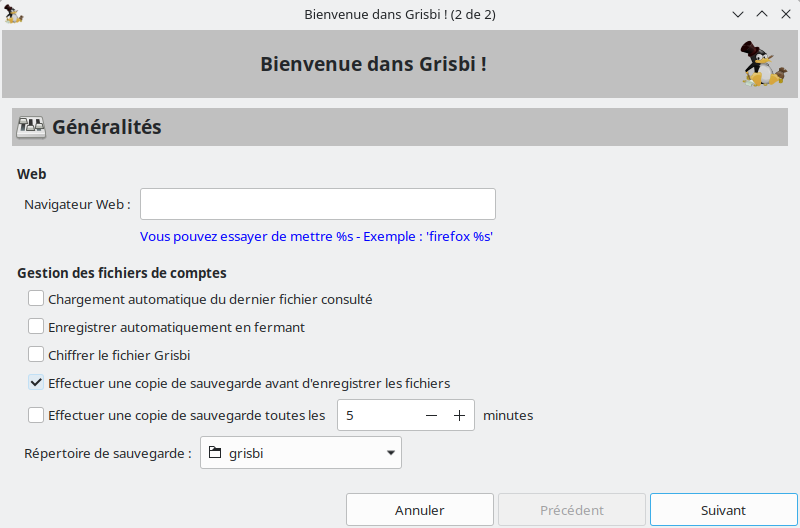
\includegraphics[width=.98\textwidth]{image/screenshot/start_first_launch}
	\end{center}
	\caption{Erstkonfiguration der Kontendatei.}
	\label{start_first_launch}
\end{figure}	
	
Es ist ratsam, die Optionen zu prüfen:%It is advisable to check the options:
	\begin{itemize}
		\item Die letzte Dateï automatisch öffnen;% Automatically load last file on startup%chargement automatique du dernier fichier consulté;
		\item Automatisch speichern;%Automatically save on exit;%enregistrer automatiquement en fermant;
		\item Vor dem Speichern eine Sicherung erstellen (standardmäßig aktiviert).%Make a backup copy before saving files (checked by default).%effectuer une copie de sauvegarde avant d'enregistrer les fichiers (coché par défaut).
	\end{itemize}
\end{enumerate}

\minisec{\textcolor{red}{\strong{Achtung:}}}
Die Grisbi-Entwickler empfehlen, die Option \menu{Datei verschlüsseln} aus den folgenden Gründen nicht zu verwenden:%The Grisbi developers recommend that you do not use the \menu{Encrypt Grisbi file} option for the following reasons:
\begin{itemize}
	\item Es gibt keine Methode zur Wiederherstellung einer verschlüsselten Datei, deren Passwort verloren gegangen ist;%there is no method for recovering an encrypted file whose password has been lost;
	\item Aus einem unbekannten Grund kann die Verwendung dieser Option unter Windows dazu führen, dass die Kontendatei völlig unbrauchbar wird.%For some unknown reason, using this option on Windows can render the accounts file completely unusable.
\end{itemize}  
Es ist jedoch ratsam, regelmäßig Sicherungskopien der unverschlüsselten Datei anzufertigen, wenn Sie sie verwenden.%However, if you use it, it is advisable to make regular back-ups of the unencrypted file.

\begin{enumerate}[resume]
	\item Der zweite Assistent, \dequote{Willkommen zu Grisbi} (oder später \dequote{Assistent für eine neue Datei}), der automatisch auf den ersten folgt, umfasst sechs Schritte, die Ihnen bei der Erstellung der \indexword{Kontodatei}\index{Kontodatei} helfen.%The second wizard, \dequote{Willkommen zu Grisbi} (or later \dequote{New file Assistant}), which automatically follows the first, includes six steps to help you create the \indexword{account file}\index{account file}.%Le deuxième assistant \frquote{Bienvenue dans Grisbi !} (ou plus tard \frquote{Aide à la création d'un nouveau fichier de comptes}), qui suit automatiquement le premier, comprend six étapes qui vous aiderons à la création du \indexword{fichier de comptes}\index{fichier de comptes}.
	\item Darauf folgt automatisch der dritte Assistent, \dequote{Ein neues Konto erstellen}, der zum Erstellen des ersten Kontos verwendet wird und im Abschnitt \ref{start-newfile} unten ausführlich beschrieben wird.%This is followed automatically by the third wizard, \dequote{Create a new account}, which is used to create the first account and is described in detail in section \ref{start-newfile} below.%Puis vient automatiquement le troisième assistant \frquote{Créer un nouveau compte} qui permet de créer le premier compte et qui est décrit en détail dans la section \ref{start-newfile} ci-dessous.
\end{enumerate}

Sie können jeden Assistenten jederzeit mit der Schaltfläche \menu{Abbrechen} verlassen.

Wenn Sie den Erststart-Assistenten nicht verwenden möchten, können Sie stattdessen eine Beispieldatei verwenden (siehe Abschnitt \ref{start-example} unten).

\section{Beispieldatei\label{start-example}}

Wenn Sie Grisbi sofort benutzen wollen, ohne die komplette Einrichtung durchlaufen zu müssen, zum Beispiel um eine Vorstellung von den Möglichkeiten dieses Programms zu bekommen, können Sie die Datei \file{Example\_3.0-de.gsb} von der \lang{Sourceforge.net}\footnote{\urlSourceForgeDocumentation{}} Website im Ordner \dequote{textsf{examples}} herunterladen.

\vspacepdf{5mm}
\textbf{Notiz}: In dieser Beispieldatei sind die Namen der Zahlungsempfänger usw. reine Erfindung; jede Ähnlichkeit mit einer realen Person oder einem realen Unternehmen ist rein zufällig.%{Note}: in this example file, the names of the payees etc are pure invention; any similarity with a real person or business is entirely accidental.

\section{Erstellen einer neuen Kontodatei\label{start-newfile}}

Wenn Sie Grisbi zum ersten Mal verwenden, müssen Sie eine erste \indexword{Kontendatei}\index{Kontendatei} erstellen. Die \gls{Dateinamenserweiterung} lautet \file{.gsb} und der Dateiname \file{Name-ihrer-Datei.gsb}.%The \gls{extension} of this file will be \file{.gsb} and its name will be \file{your-file-name.gsb}.

Unmittelbar danach müssen Sie mindestens ein Konto (Bank-, Geld-, Passiv- oder Aktivkonto, beschrieben im Kapitel Kontoverwaltung) und einige weitere Konten (Giro-, Spar-, Kredit-, eventuell ein \vref{accounts} \menu{Verwaltung von Konten} und einige Übergangskonten) anlegen, die ihre jeweiligen Transaktionen enthalten werden.%Immediately afterwards, you will need to create at least one account (bank, cash, liability or asset account, described in the chapter \vref{accounts} \menu{Account management}), and then a few other accounts (current, savings, credit, possibly a cash account and a few transition accounts) which will contain their respective transactions.

Bei einer Familienverwaltung haben Sie normalerweise nur eine einzige Kontodatei, da dies den gesamten Austausch zwischen Ihren verschiedenen Konten ermöglicht. Wenn Sie einen Verein oder eine weitere Familie verwalten, die in keinem buchhalterischen Zusammenhang mit der ersten Familie steht, erstellen Sie eine weitere Kontodatei, die einen anderen Namen trägt \file{name-ihrer-zweiten-datei.gsb}. Dadurch bleiben die \indexword{Buchhaltungseinheiten}\index{Buchungsberechtigung} getrennt. %If you are managing a family, you will normally only have one accounts file, as this allows all the exchanges between your different accounts. If you are managing an association, or another family with no accounting relationship with the first, you will create another accounts file, which will have a different name your-second-file-name.gsb. This will keep the \indexword{accounting entities}\index{accounting entity} separate.

Mit anderen Worten: Alle Konten Ihres Haushalts werden in einer Kontendatei erfasst, alle Konten Ihrer Vereinigung in einer anderen Kontendatei.



%\cleardoubleemptypage

%%%%%%%%%%%%%%%%%%%%%%%%%%%%%%%%%%%%%%%%%%%%%%%%%%%%%%%%%%%%%%%%%
% Contents: The home chapter
% $Id: grisbi-manuel-home.tex, v 0.4 2002/10/27 Daniel Cartron
% $Id: grisbi-manuel-home.tex, v 0.5.0 2004/06/01 Loic Breilloux
% $Id: grisbi-manuel-home.tex, v 0.6.0 2011/11/17 Jean-Luc Duflot
% some of its content was in menus chapter:
% $Id: grisbi-manuel-menus.tex, v 0.5.0 2004/06/01 Loic Breilloux
% $Id: grisbi-manuel-home.tex, v 0.8.9 2012/04/27 Jean-Luc Duflot
% $Id: grisbi-manuel-home.tex, v 1.0 2014/02/12 Jean-Luc Duflot
%%%%%%%%%%%%%%%%%%%%%%%%%%%%%%%%%%%%%%%%%%%%%%%%%%%%%%%%%%%%%%%%%

\chapter{Eintritt in Grisbi\label{entrance}}%Entrée dans Grisbi%Entering Grisbi

\section{Auswahl einer Datei\label{select-file}}%Sélection d'un fichier%Selecting a file

\vspacepdf{3mm}			% vertical space = 5 mm

Wenn Sie die Anwendung starten, zeigt Grisbi eine Seite an, die es Ihnen ermöglicht, auf verschiedene Weise zu beginnen.%When you launch the application, Grisbi displays a page allowing you to get started in different ways.%Au lancement de l'application, Grisbi affiche la page qui vous permet de démarrer de différentes manières.

\vspacepdf{3mm}			% espace: 5 mm

Sie können das Grisbi-Fenster in \indexword{Vollbild}\index{Anzeige!Vollbild}\index{Vollbild!Anzeige} durch Drücken der Funktionstaste \key{F11} anzeigen und mit derselben Taste zurückgehen.%You can display the Grisbi window in \indexword{full screen}\index{display!full screen}\index{full screen!display} by pressing the function key \key{F11}, and go back using the same key.%Vous pouvez afficher la fenêtre de Grisbi en \indexword{plein écran}\index{affichage!plein écran}\index{plein écran!affichage} par la touche de fonction \key{F11}, et revenir en arrière par la même touche.			% "!" separates the term from the subterm of the index entry

\vspacepdf{3mm}			% espace: 5 mm

\begin{figure}[htbp]			% h=here, t=top, b=bottom, p=page of float to force the figure here, not in a next page.
	\begin{center}					% image centrée
		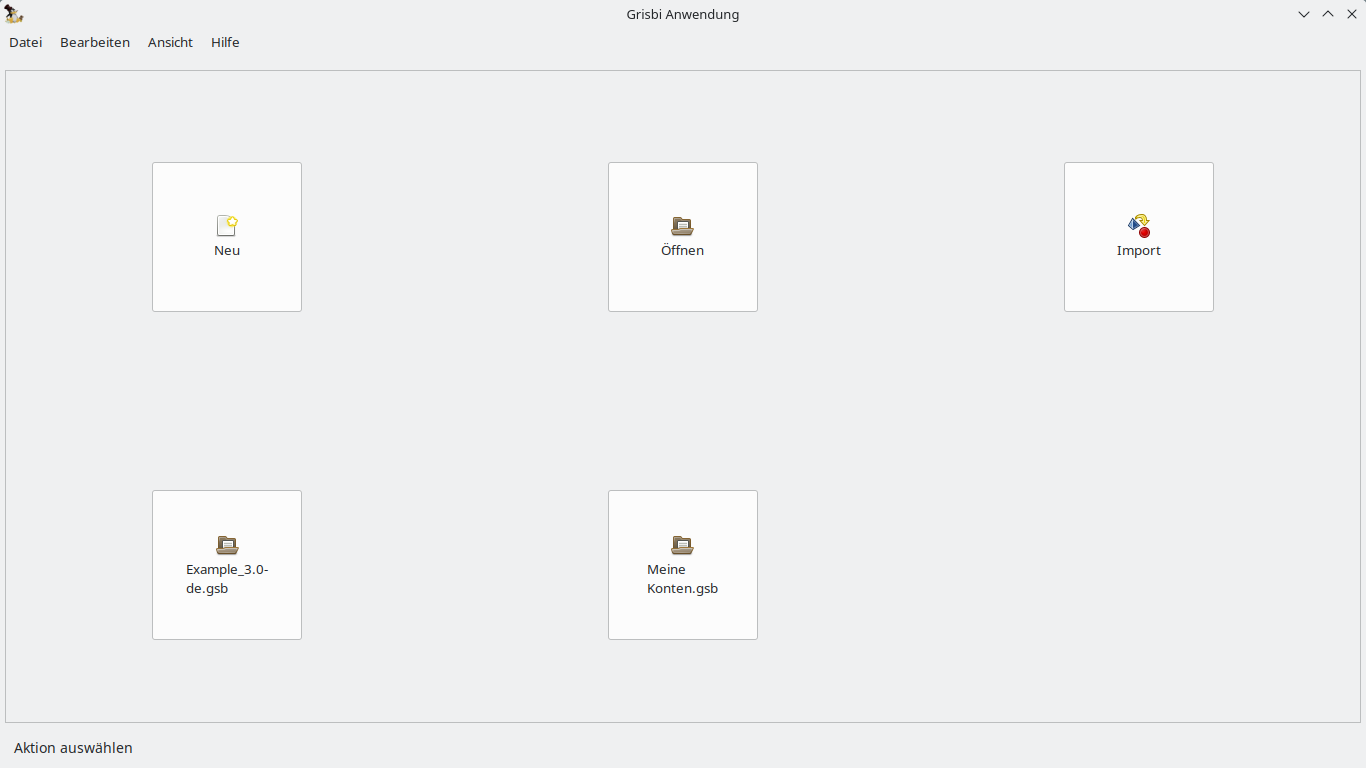
\includegraphics[width=0.95\textwidth]{image/screenshot/home_start_grisbi}		% width=95% as wide as the current text
	\end{center}
	\caption{Startfenster}%Start-up window}%Fenêtre de démarrage}			% sous-titre/subtitle
	\label{home_start_grisbi}					% figure's ref., use for link in text with \refimage{}
\end{figure}

\vspacepdf{3mm}			% espace: 5 mm

Neben der Menüleiste enthält dieses Fenster eine Reihe von Bedienfeldern:%In addition to the menu bar, this window displays a number of panels:%En plus de la barre de menu, cette fenêtre affiche plusieurs pavés:

\begin{itemize}
	\item die Schaltfläche \dequote{Neu}, um den Assistenten \dequote{Assistent für neue Datei} zu starten;%le pavé Nouveau, pour lancer l'assistant \frquote{Aide à la création d'un nouveau fichier de comptes};
	\item die Schaltfläche \dequote{Öffnen}, um einen Dateimanager anzuzeigen, mit dem Sie nach einer vorhandenen Kontendatei auf Ihrem Computer suchen können;%le pavé Ouvrir, pour afficher un gestionnaire de fichier avec lequel vous pourrez chercher un fichier de comptes existant dans votre ordinateur;
	\item die Schaltfläche {Import}, um den Assistenten {Assistent für eine neue Datei mittels Import} zu starten;%le pavé \frquote{Importer}, pour lancer l'assistant \frquote{Importation des opérations par Grisbi};
	\item eine oder mehrere weitere Schaltflächen, die nach Kontodateien benannt sind, die Grisbi bereits verwendet hat.%un ou plusieurs autres pavés, portant le nom de fichiers de comptes que Grisbi a déjà utilisés.
\end{itemize}

\vspacepdf{5mm}

\textbf{Notiz}: Schaltflächen mit den Namen von Kontodateien, die Grisbi bereits verwendet hat, sind nur vorhanden, wenn diese Dateien existieren; wenn Sie sie von dieser Eingabeseite entfernen möchten, verschieben Sie sie in ein anderes Verzeichnis oder löschen Sie sie.%les pavés portant les noms des fichiers de comptes que Grisbi a déjà utilisés ne sont présents que si ces fichiers existent; si vous voulez les enlever de cette page d'entrée, déplacez-les dans un autre répertoire, ou supprimez-les.

\vspacepdf{3mm}			% espace: 5 mm

Unten auf der Seite werden Sie durch ein Banner aufgefordert, eine Aktion auszuwählen, indem Sie eine dieser Schaltflächen wählen.%En bas de page, un bandeau vous appelle à choisir une action en sélectionnant l'un de ces pavés.

\vspacepdf{3mm}			% espace: 5 mm

Wenn Sie die Grisbi-Software nur kennenlernen möchten, um eine Vorstellung davon zu bekommen, wie sie aussieht und was sie kann, können Sie stattdessen eine Beispieldatei wie die auf der Website \lang{Sourceforge.net}\footnote{\urlSourceForgeDocumentation{}} im Ordner \dequote{examples} verwenden.%Si vous voulez juste découvrir le logiciel Grisbi pour avoir un aperçu de son aspect et de ses possibilités, vous pouvez à la place utiliser un fichier exemple comme celui présent sur le site de \lang{Sourceforge.net}\footnote{\urlSourceForgeDocumentation{}} dans le dossier \frquote{\textsf{examples}}.		% (voir la section \vref{new-example}).

\vspacepdf{5mm}			% espace: 5 mm

\textbf{Notiz}: Durch einfaches Anklicken der heruntergeladenen Beispieldatei wird Grisbi gestartet und zeigt das Home-Fenster\refimage{home_3.0} direkt an, ohne das Startfenster zu durchlaufen.%en cliquant simplement sur le fichier exemple téléchargé, Grisbi s'exécutera en affichant directement la fenêtre d'accueil\refimage{home_3.0} sans passer par la fenêtre de démarrage.

\section{Startseite\label{home}}%Homepage%Accueil

\vspacepdf{3mm}

Wenn eine Kontodatei geöffnet wird, zeigt Grisbi die Startseite\refimage{home_3.0} an.%When an account file is opened, Grisbi displays its home page\refimage{home_3.0}.%When the application starts, Grisbi displays this
Dies ist die Startseite des Programms, auf die Sie jederzeit durch Klicken auf die Registerkarte \menus{Konten} zugreifen können.%This is the start page of the programme and can be accessed at any time by clicking on the \menus{Accounts} tab.

\vspacepdf{3mm}

\begin{figure}[htbp]			% h=here, t=top, b=bottom, p=page of float to force the figure here, not in a next page.
	\begin{center}
		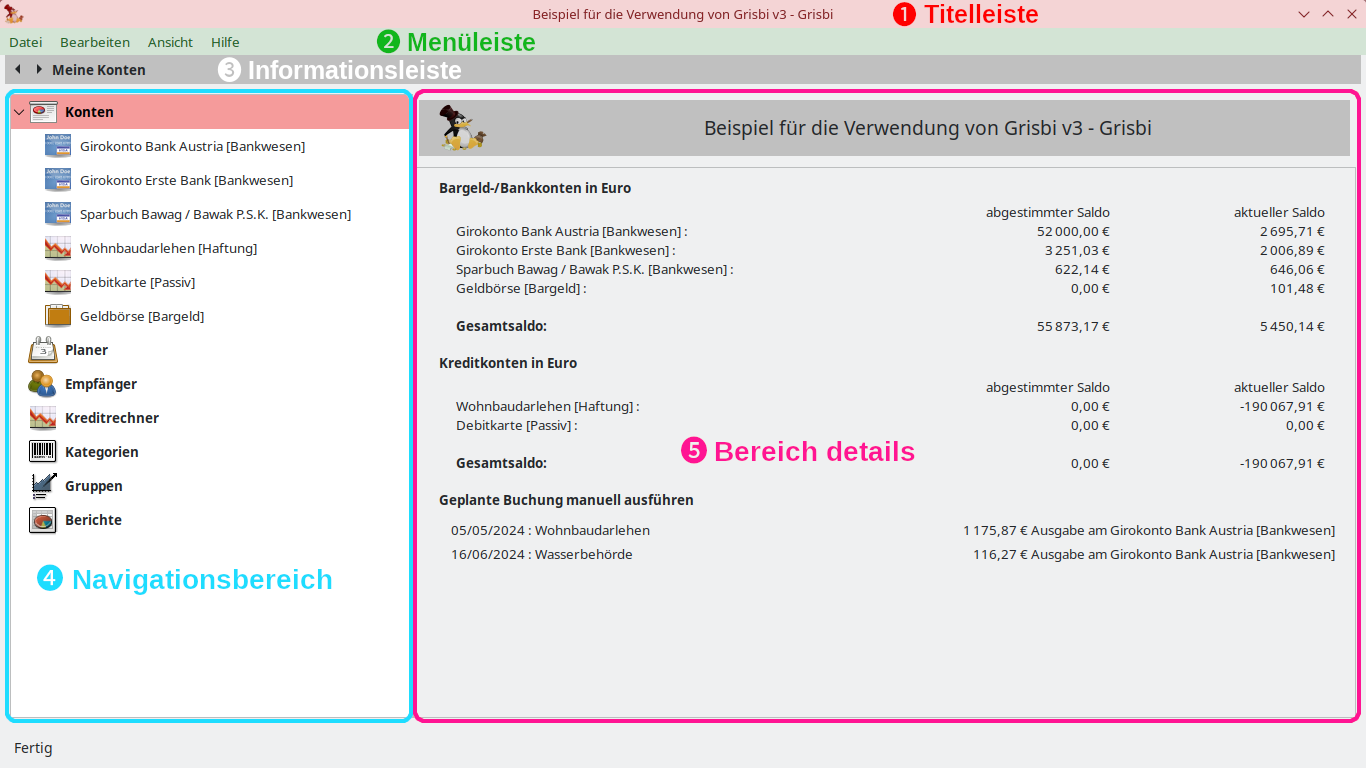
\includegraphics[width=1\textwidth]{image/screenshot/home_3.0.png}
	\end{center}
	\caption{Kontenübersichtsseite}		% sous-titre/subtitle
	\label{home_3.0}
\end{figure}

\vspacepdf{3mm}

Grisbi zeigt alle Seiten auf die gleiche Weise an: Wie jede Software zeigt sie an:%Alle Grisbi-Bildschirme haben das gleiche allgemeine Aussehen. Er zeigt eine Menüleiste, die Zugang zu den meisten wichtigen Funktionen von Grisbi bietet, sowie drei Hauptbereiche:%All Grisbi screens have the same general appearance. It displays a menu bar that gives access to most of Grisbi's important features, and three main areas:

\begin{itemize}%[\large \textcircled{\small 2}]
	\item[\large\textcircled{\small 1}] die Titelleiste;%une barre de titre;
	\item[\large\textcircled{\small 2}] die Menüleiste, die Zugang zu den meisten wichtigen Funktionen der Grisbi bietet;%une barre de menus qui donne accès à la plupart des fonctionnalités importantes de Grisbi;
\end{itemize}
sowie drei Grisbi spezifische Bereiche:%as well as three specific Grisbi zones:%et aussi trois zones qui sont spécifiques à Grisbi:
\begin{itemize}%[3,4,5]
	\item[\large\textcircled{\small 3}] die Informationsleiste unter der Menüleiste;%la barre d'information, sous la barre de menus;
	\item[\large\textcircled{\small 4}] die Navigationsbereich;%le panneau de navigation;
	\item[\large\textcircled{\small 5}] die Bereich details%le panneau des détails
\end{itemize}

\section{Informationsleiste\label{home-synthesis}}

Die Informationsleiste zeigt den Namen der aktuell ausgewählten Registerkarte an und kann ganz rechts bestimmte Bilanzen anzeigen, die sich auf das beziehen, was im Detailbereich ausgewählt wurde.%The information bar shows the name of the currently selected tab select tab di can display, completely to the right, certain balances relating to what is selected in the details panel.

\vspacepdf{5mm}

\textbf{Notiz}: die standardmäßig angezeigte Informationsleiste kann durch Deaktivieren eines Kontrollkästchens in den Einstellungen \vref{setup-display-toolbars} ausgeblendet werden.%\textbf{Note}: the information bar, displayed by default, can be hidden by unchecking a box in the preferences \vref{setup-display-toolbars}.
\vspacepdf{3mm}

Um eine der in der Navigationsleiste angezeigten Registerkarten auszuwählen, klicken Sie einmal oder mehrmals auf eines der beiden kleinen Dreiecke oben links in der Leiste.  Die angezeigten Elemente sind: \menus{Konten}, \menus{Planer}, \menus{Empfänger}, \menus{Kreditrechner}, \menus{Kategorien}, \menus{Gruppen} und \menus{Berichte}.  Wenn die Elemente \menus{Konten} und \menus{Berichte} erweitert wurden, um ihre Unterkategorien anzuzeigen, werden diese auch einzeln angezeigt.%To select one of the tabs displayed in the navigation panel click one or more times on one of the two small triangles on the top left of the panel.  The items displayed are: \menus{Accounts}, \menus{Scheduler}, \menus{Payees}, \menus{Credits simulator}, \menus{Categories}, \menus{Budgetary lines} and \menus{Reports}.  If the \menus{Accounts} and \menus{Reports} items have been expanded to display their sub categories these will also be displayed one by one.

\vspacepdf{5mm}

\textbf{Notiz}: Je nach dem Thema der Desktop-Umgebung oder des Fenstermanagers, die Sie verwenden, können diese dreieckigen Symbole durch andere Zeichen wie +, -, >, < usw. ersetzt werden.%Depending on the theme of the desktop environment or window manager you are using, these triangular symbols might be replaced by other characters such as +, -, >, <, etc.

\vspacepdf{3mm}
Der Inhalt der Auswahl wird im Bereich details angezeigt.%The content of the selection is displayed in the main screen area.

\vspacepdf{3mm}
Diese Funktionen können anstelle des Navigationsbereich verwendet werden, wenn dessen Breite auf Null reduziert ist und Sie keinen direkten Zugang zu ihm haben.%These functions can be used in place of the navigation panel when its width is reduced to zero and you do not have direct access to it.


\section{Navigationsbereich\label{home-accounting}}

\begin{wrapfigure}{l}{0.33\textwidth}%50mm}
\vspace{-\intextsep}				% space above the floating (minus intextsep=separation between float and text in text)
\centering							% centering the floating figure in the "wrap"
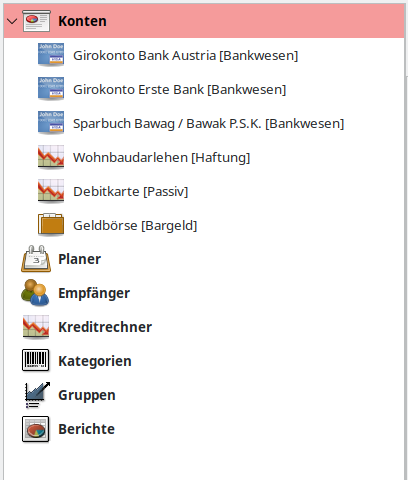
\includegraphics[width=0.28\textwidth]{image/screenshot/home_navigation}
\vspace{-5pt}						% space between the floating and the caption below the floating
\captionsetup{%						% for a change of options of the caption package
	format=plain,					% to avoid error message with labelsep option below, default=hang
	name=Abb.,						% rename label caption, default="Figure" (or "Table")
	justification=centering,		% centring of text and caption label 
	labelsep=newline				% define the separator between the label and the caption text
}
\caption{Navigationsbereich}		% \caption is mandatory to reference a figure in lof
\vspace{-40pt}						% space below the caption
\label{home_navigation}
\end{wrapfigure}

Im Navigationsbereich wird die Liste der Registerkarten in Fettdruck angezeigt:
	\begin{itemize}
		\item \menus{Konten}%Accounts},
		\item \menus{Planer}%Scheduler},
		\item \menus{Empfänger}%Payees},
		\item \menus{Kreditrechner}%Credits simulator},
		\item \menus{Kategorien}%Categories},
		\item \menus{Gruppen}%Budgetary lines},
		\item \menus{Berichte}%Reports}.
	\end{itemize}
Wenn Sie auf das kleine schwarze Dreieck links neben den Registerkarten \menus{Konten} oder \menus{Berichte} klicken, können Sie die Liste der Unterregisterkarten durchblättern oder aufrollen. Sie können die Reihenfolge der Registerkarten und Unterregisterkarten ändern, indem Sie auf eine von ihnen klicken und sie in der Liste nach oben oder unten ziehen.%By clicking on the small black triangle to the left of the  \menus{Accounts} or \menus{Reports} tabs,  you can scroll or roll up the list of their sub-tabs. You can change the order of tabs and sub-tabs by clicking on one of them and dragging it up or down the list.

\vspacepdf{5mm}

\textbf{Notiz}:  Je nach dem Thema der Desktop-Umgebung oder des Fenstermanagers, die Sie verwenden, können diese dreieckigen Symbole durch andere Zeichen wie +, -, >, < usw. ersetzt werden.%These triangles can be replaced, depending on the theme of the desktop environment or window manager you are using, by other characters such as +, -,>, <, and so on.

\vspacepdf{3mm}

Sie können eine dieser Registerkarten oder Unterregisterkarten auswählen, indem Sie auf ihren Namen klicken. Sie können die Auswahl in dieser Liste von Registerkarten und Unterregisterkarten auch mit den \keys{Pfeiltasten Hinauf}, \keys{Pfeiltasten Herunter}, \keys{Bild Hinauf} oder \keys{Bild Herunter} oder mit dem Mausrad verschieben (diese Option muss in den Voreinstellungen \vref{setup-display-toolbars} aktiviert werden).%You can select one of these tabs or sub-tabs by clicking on its name. You can also move the selection in this list of tabs and sub-tabs with the \key{Up Arrow}, \key{Down Arrow}, \key{Page Up} ou \key{Page Down} keys, or with the mouse wheel (option to be checked in the preferences \vref{setup-display-toolbars}). 

\vspacepdf{3mm}
Der Inhalt der Auswahl wird im Bereich details angezeigt.%The contents of the selection are displayed in the details panel.

\vspacepdf{3mm}

Sie können die Breite des Navigationsbereich verkleinern oder vergrößern, indem Sie auf den dünnen vertikalen Balken zwischen diesem Fenster und dem Bereich details klicken und ihn verschieben. Wenn die Breite des Fensters auf Null reduziert oder auf die maximale Breite des Grisbi-Fensters vergrößert wurde, kann sich die dünne vertikale Leiste links oder rechts vom Fenster befinden.  Suchen Sie diesen und schieben Sie ihn an die gewünschte Stelle zurück.%You can reduce or enlarge the width of the navigation panel by clicking on the thin vertical bar between this panel and the details panel, and moving it. If the width of the window has been reduced to zero, or enlarged to the maximum of the width of the Grisbi window, the thin vertical bar may be to the left or to the right of the window.  Locate this and slide it back to the desired location.

\vspacepdf{3mm}

Die \indexword{Kontextmenüs}\index{Kontextmenü}, die durch einen Rechtsklick mit der Maus zugänglich sind, sind auf den Elementen dieses Bereich verfügbar und bieten die folgenden Funktionen:%The \indexword{context menus}\index{context menus}, accessible by a right-click of the mouse, are available on the elements of this panel and offer the following functions:

\begin{itemize}
	 \item Auf \menus{Konten}%Accounts}:
		\begin{itemize}
			 \item \menus{Konto erstellen}%New account};
		\end{itemize}
	 \item Erfasste Konten:%On any account: 
		\begin{itemize}
			 \item \menus{Konto erstellen}%New account},
			 \item \menus{Konto löschen}%Remove this account};
		\end{itemize}
	 \item Auf \menus{Empfänger}%Payees}:
		\begin{itemize}
			 \item \menus{Empfänger erstellen}%New payee},
			 \item \menus{Den ausgewählten Empfänger löschen}%Delete selected payee},
			 \item \menus{Den ausgewählten Empfänger bearbeiten}%Edit selected payee},
			 \item \menus{Empfänger verwalten}%Manage payees},
			 \item \menus{Verwaiste löschen}%Remove unused payees};
		\end{itemize}
	 \item Auf \menus{Kategorien}%Categories}: 
		\begin{itemize}
			 \item \menus{Kategorie erstellen}%New category},
			 \item \menus{Die ausgewählten Kategorie löschen}%Delete selected category},
			 \item \menus{Die ausgewählte Kategorie bearbeiten}%Edit selected category},
			 \item \menus{Kategorien (*.csgb) importieren}%Import a file of categories (.csgb)},
			 \item \menus{Kategorien (*.csgb) exportieren}%Export the list of categories (.csgb)};
		\end{itemize}
	 \item Auf \menus{Gruppen}%Budgetary lines}:
		\begin{itemize}
			 \item \menus{Gruppe erstellen}%New budgetary line},
			 \item \menus{Die ausgewählten Gruppe löschen}%Delete selected budgetary line},
			 \item \menus{Die ausgewählte Gruppe bearbeiten}%Edit selected budgetary line},
			 \item \menus{Gruppen (*.isgb) importieren}%Import a file of budgetary lines (*.isgb)},
			 \item \menus{Gruppen (*.isgb) exportieren}%Export the list of budgetary lines (*.isgb)};
		\end{itemize}
	 \item Auf \menus{Berichte}: \menus{Bericht erstellen};%New report}%Report}: \menus{New report};
	 \item Auf Erfasste Berichte:%any report: 
		\begin{itemize}
			 \item \menus{Bericht erstellen}%New report},
			 \item \menus{Den ausgewählten Bericht löschen}%Remove this report}.
		\end{itemize}
\end{itemize}

\section{Bereich details\label{home-details}}

Das Bereich details zeigt alle Details zu den über die Informationsleiste oder das Navigationsbereich ausgewählten Registerkarten oder Unterregisterkarten an. Dies ist der Hauptarbeitsbereich von Grisbi.

Sie können es verkleinern oder vergrößern, indem Sie auf die dünne vertikale Leiste zwischen diesem Fenster und dem Navigationsbereich klicken und sie ziehen. Wenn die Breite dieses Fensters auf Null reduziert oder auf die maximale Breite des Grisbi-Fensters vergrößert wurde, kann sich die dünne vertikale Leiste links oder rechts vom Fenster befinden. Suchen Sie diesen und schieben Sie ihn an die gewünschte Stelle zurück.%The details panel displays all the details on the tabs or sub-tab selected by the Information bar or Navigation panel. This is the main work area of Grisbi.
%You can reduce or enlarge its width by clicking on the thin vertical bar between this window and the navigation panel, and dragging it. If the width of the this panel has been reduced to zero or enlarged to the maximum of the width of the Grisbi window, the thin vertical bar may be to the left or to the right of the window.  Locate this and slide it back to the desired location.

\begin{figure}[htbp]			% h=here, t=top, b=bottom, p=page of float to force the figure here, not in a next page.
	\begin{center}
		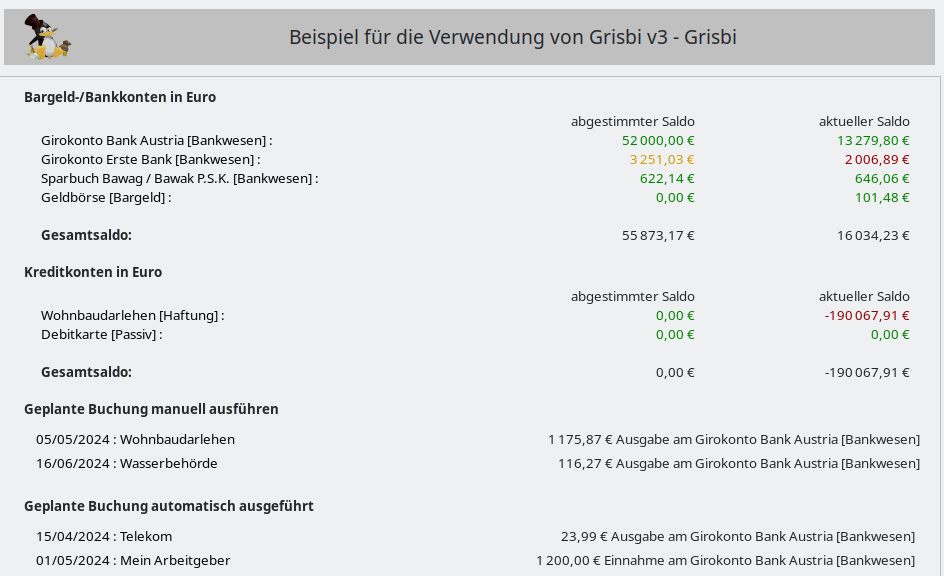
\includegraphics[width=1\textwidth]{image/screenshot/home_details.png}
	\end{center}
	\caption{Geändertes Bereich details}		% sous-titre/subtitle
	\label{home_details}
\end{figure}
 
\subsection{Anzeige von Details auf der Startseite\label{home-details-homepage}}

Wenn Sie die Registerkarte \menus{Konten} auswählen, wird das Bereich details angezeigt:%By selecting the \menus{Accounts} tab, the details panel displays:

\begin{itemize}
	\item in einem grauen Hintergrundbanner nach oben:%to the top in a grey background banner:
		\begin{itemize}
			\item das \menus{Grisbi}-Symbol (das ausgeblendet werden kann, siehe \vref{setup-display-logo-icon}),
			\item und auf der rechten Seite den \indexword{Titel}\index{Titelanzeige!Titel}\index{Hauptseite} der aktuell geladenen Buchhaltungsdatei in der Form \dequote{zugewiesener Name - Grisbi}; Sie können diese Bezeichnung unter drei Möglichkeiten im Menü \menus{Bearbeiten - Einstellungen} festlegen (siehe den Abschnitt \vref{setup-display-addresses-titles}, Adressen \& Bezeichnungen):%in a box on a gray background, on the left, the \menus{Grisbi} icon (which can be hidden, see \vref{setup-display-logo-icon}) and on the right the \indexword{title}\index{title display!title}\index{home page} of the accounts file you currently have loaded, in the form \enquote{assigned name - Grisbi}; you can define this label, from among three possibilities, in the \menus{Edit preferences} menu (see the paragraph \vref{setup-display-addresses-titles}):
				\begin{itemize}
			 		\item die \menus{Bezeichnung} (standardmäßig): Dies ist der Name, den Sie zur Identifizierung der Art des Kontos verwenden, z. B. \dequote{Meine Konten} oder \dequote{Business}, den Sie bei der Erstellung der Kontodatei eingegeben haben; Sie können ihn hier im Feld \menus{Bezeichnung} bearbeiten; dies kann nützlich sein, wenn Sie mehrere \indexword{Bezeichnungen}\index{Bezeichnung} verwalten,%the \menus{Accounting entity}: This is the name you use to identify the type of account e.g. \enquote{My Accounts} or \enquote{Business}, which you entered when the account file was created; you can edit it here in the \menus{Name of accounting entity} field; this can be useful if you manage multiple \indexword{accounting entities}\index{accounting entity}, 
					\item die \menus{Kontoinhaber}: den Namen des Inhabers (oder des Kontoverwalters) des zuletzt aufgerufenen Kontos; wenn der Inhaber nicht in den Kontoeigenschaften definiert ist, zeigt Grisbi den Namen dieses Kontos an,%the \menus{Account owner name}: the name of the owner (or  account manager) of the last account accessed; if the holder is not defined in the account properties, Grisbi displays the name of this account,
			 		\item die \menus{Dateiname}: Dies ist der Name der Datei im aktuellen Verzeichnis in der Form \file{Name\_deiner\_Datei.gsb};%the \menus{Filename}: this is the name of the file in the current directory, in the form \file{name\_of\_your\_file.gsb};
			 	\end{itemize}
		\end{itemize}
	\item im hellgrauen Hauptbereich unterhalb des Banners:%in the main light grey area below the banner:
	 	\begin{itemize}
	 		\item für jede Währung getrennt, für alle Konten und \indexword{Kontengruppen}\index{Kontengruppe}, unter den Bezeichnungen \menus{abgestimmter Saldo} und \menus{aktueller Saldo}:%for each currency separately, for all accounts and \indexword{groups of accounts}\index{groupe de comptes},  under the label \menus{Reconciled balance} and \menus{Current balance}:
				\begin{itemize}
					\item den Saldo der Bank- und Kassenkonten, den Teilsaldo der Kontengruppen und deren Gesamtsaldo,%the balance of the bank and cash accounts, the partial balance of the groups of accounts and their global balance,
					\newline
					\textbf{Notiz}: können Sie die Reihenfolge der Anzeige der Teilsalden der Kontengruppen anpassen (siehe Abschnitt \vref{setup-general-home-partBalance}, Teilweise Salden der Kontenliste)%you can adjust the display order of the partial balances of the account groups (see the section \vref{setup-general-home-partBalance}, \menus{Partial balances of the list of accounts}).			 
					\item der Saldo der Passivkonten und ihr Endsaldo,%the balance of the liability accounts and their final balance,
					\item der Saldo der Vermögenskonten und ihr Endsaldo;%the balance of the asset accounts and their final balance;
				\end{itemize}
			\item die \indexword{Warnungen vor automatisch geplanten Einträgen}\index{Warnung!geplanter Eintrag} mit ihrem Datum, entsprechend der im \menus{Bearbeiten - Einstellungen} getroffenen Auswahl (siehe den Abschnitt \vref{Einrichten - Allgemeiner Plan}, \menus{Planer}),%the \indexword{alerts from automatically scheduled entries}\index{alert!scheduled entry} with their date, wording and amount, according to the choices made in the \menus{Edit - Preferences} menu (see the section \vref{setup-general-planned}, \menus{Timetable});
			\item die Liste der Konten, deren Saldo unter den \menus{Mindestsaldo zulässig} gefallen ist,%the list of accounts whose balance has fallen below the \menus{Minimum authorized balance};
			\item die Liste der Konten, deren Saldo unter den \menus{Mindestsaldo festgelegt} gefallen ist.%the list of accounts whose balance has fallen below the \menus{Minimum desired balance}.
		\end{itemize}
\end{itemize}

\vspacepdf{5mm}

\textbf{Notiz}: Definitionen der Begriffe \menus{Mindestsaldo zulässig} und \menus{Mindestsaldo festgelegt} finden Sie im Abschnitt \vref{accounts-properties}, \menus{Konten bearbeiten}.%For definitions of \menus{Minimum authorized balance} and \menus{Minimum desired balance}, see the \vref{accounts-properties}, \menus{Account Properties} section.

\vspacepdf{3mm}

Die Kontobezeichnungen werden in \textcolor{black}{schwarz} angezeigt. Wenn Sie den Mauszeiger über eine dieser Zeilen bewegen, ändert sich ihre Farbe in \textcolor{gray}{grau}.%The account labels are displayed in \textcolor{black}{schwarz}; as the mouse cursor moves over the line of one of these, its colour changes to \textcolor{gray}{grau}.

Eine Balance, die größer ist als die \menus{Mindestsaldo festgelegt}, wird in \textcolor[RGB]{0,126,0}{grün} angezeigt: Wenn sich der Cursor über die Zeile bewegt, ändert sich ihre Farbe in \textcolor[RGB]{0,227,0}{hellgrün}.%A balance greater than the \menus{Minimum desired Balance} is displayed in \textcolor[RGB]{0,126,0}{green}: as the cursor moves over the line, its colour changes to \textcolor[RGB]{0,227,0}{light green}.

Ein Saldo, der kleiner als der {Mindestsaldo festgelegt} und größer als der {Mindestsaldo zulässig} ist, wird in \textcolor[RGB]{230,155,0}{orange} angezeigt: wenn der Zeiger auf seiner Linie vorbeigeht, ändert sich diese Farbe zu \textcolor[RGB]{255,200,0}{hellorange}.%A balance less than the \menus{Minimum desired balance} and greater than the \menus{Minimum authorized balance} is displayed in \textcolor[RGB]{230,155,0}{orange}: as the pointer passes on its line, this color changes to \textcolor[RGB]{255,200,0}{light orange}.

Ein Saldo, der kleiner ist als der {Mindestsaldo zulässig}, wird in \textcolor[RGB]{153,0,0}{Dunkelrot} angezeigt: wenn der Zeiger über die Linie fährt, ändert sich diese Farbe zu \textcolor{red}{red}.%A balance less than the  \menus{Minimum authorized Balance}  is displayed in \textcolor[RGB]{153,0,0}{dark red}: as the pointer passes over its line, this color changes to \textcolor{red}{red}.

Wenn Sie den Mauszeiger über die Zeile eines Kontos bewegen, zeigt jede Farbänderung an, dass die im markierten Konto enthaltenen Datensätze angezeigt werden, wenn Sie mit der Maus klicken (rechts oder links), als ob das Konto mit der Informationsleiste oder dem Navigationsbereich ausgewählt worden wäre.%When you move the mouse pointer over the line of an account, any color change indicates that if you click (right or left) with the mouse, the records contained in the highlighted account is displayed, as if the account had been selected with the information bar or navigation panel.

Ein Teilsaldo kann für eine Gruppe von Konten angegeben werden. Ist er definiert, wird er in \textcolor[RGB]{40,40,255}{dunkelblau} angezeigt (wie in der Abbildung \vref{home_details}). Wenn er negativ ist, kann er in \textcolor[RGB]{153,0,0}{dunkelrot} erscheinen (siehe \vref{setup-general-home-partBalance}, \menus{Teilsalden}). Eine Teilbilanzzeile ändert ihre Farbe nicht, wenn der Mauszeiger über ihr steht, da Sie die einzelnen Einträge einer Kontengruppe nicht sehen können.%A partial balance can be specified for a group of accounts  If defined this is displayed in \textcolor[RGB]{40,40,255}{dark blue} (see the example in the figure \vref{home_details}). If it is negative, it may appear in \textcolor[RGB]{153,0,0}{dark red}, (see  \vref{setup-general-home-partBalance}, \menus{Balances partials of the list of accounts}). A partial balance line does not change color when the mouse pointer is over it, because you can not view the individual entries for of an group of accounts.

% espace pour changement de thème
\vspacepdf{3mm}
Sie können bestimmte Aspekte der Anzeige des Bereich details konfigurieren:%You can configure certain aspects of the display of the details panel:
\begin{itemize}
	\item in the \menus{Bearbeiten - Einstellungen} menu: %TODO verify sections/paragraphs with \vref{setup-xxx}
	\begin{itemize}
		\item \menus{\indexword{Allgemein}\index{allgemein}}:
		\begin{itemize}
			\item \menus{Allgemeines}, tab \menus{Planer}\index{planer}: Abschnitt \vref{setup-general-planned};
			\item \menus{Startseite}:
			\begin{itemize}
				\item \menus{Berechnung der Salden}: Absatz \vref{setup-general-home-balance},
				\item \menus{Teilsalden}: Absatz \vref{setup-general-home-partBalance};
			\end{itemize}
		\end{itemize}
		\item \menus{\indexword{Anzeigeoptionen}\index{anzeigeoptionen}}:
		\begin{itemize}
			\item \menus{Schriften \& Logo}\index{Schriften}\index{logo}: Abschnitt \vref{setup-display-logo},
			\item \menus{Adressen \& Bezeichnungen}\index{bezeichnunge}\index{adresse}: Abschnitt \vref{setup-display-addresses-titles};
		\end{itemize}
	\end{itemize}
	\item auf der tab \menus{Eigenschaften} der einzelnen Konten in der Rubrik \menus{Saldoinformationen}:%in the \menus{Properties} tab of each account:
	\begin{itemize}
		\item Konten unterhalb des \menus{Mindestsaldo zulässig}\index{saldo!mindest zulässig}: Abschnitt \vref{accounts-properties}:
		\item Konten unterhalb des \menus{Mindestsaldo festgelegt}\index{saldo!mindest festgelegt}: Abschnitt  \vref{accounts-properties}.
	\end{itemize}
\end{itemize}

%In particular, if you find a spelling error in this page, you can correct it: see the paragraph \vref{setup-general-home-final}, \menus{?? Pluriel de final ??} !

\section{Menüleiste\label{home-menus}}

Wie in vielen Grafikanwendungen sind die meisten wichtigen Funktionen von Grisbi über die Menüs in der \indexword{Menüleiste}\index{Menüleiste} zugänglich. Die Funktionen werden im Folgenden detailliert beschrieben.%As in many graphics applications, most of Grisbi's important features are accessible through the menus in the \indexword{Menu Bar}\index{barre de menus}. The features are detailed below.


\subsection{Menü \menus{Datei}\label{home-menus-file}}

Dieses Menü enthält die folgenden Funktionen:%This menu includes the following functions:

\vspace{3mm}
\begin{itemize}[rightmargin=.6cm]
	\item \menus{Neues Fenster}: nicht funktionsfähig (vielleicht in Zukunft?)%TODO: to update
	%non-functional (perhaps in the future?)
\end{itemize}

\noindent
\begin{minipage}{.7\linewidth}
	\begin{itemize}[rightmargin=.6cm]
		\item \menus{Neu}: erstellt eine neue Grisbi-Datei mit der \gls{Dateinamenserweiterung} \file{.gsb}; die aktuelle Datei wird daher geschlossen und eine neue leere Datei mit einem leeren Konto erstellt (Tastenkombination \keys{Strg+N}), siehe den Abschnitt \vref{start-newfile}; nicht zu verwechseln mit der Erstellung eines neuen Kontos;%creates a new Grisbi file of \gls{extension}\file{.gsb}; the current file is therefore closed and a new empty file is created with an empty account (shortcut \keys{Ctrl+N}), see the section \vref{start-newfile}; not to be confused with the creation of a new account;%\menus{Nouveau fichier de comptes}: crée un nouveau fichier Grisbi d'\gls{extension} \file{.gsb}; le fichier courant est donc fermé et un nouveau fichier vide est créé avec un compte vide (raccourci-clavier \keys{Ctrl+N}), voir la section \vref{start-newfile}; à ne pas confondre avec la création d'un nouveau compte;	 
		\item \menus{Öffnen}: öffnet Ihren Dateimanager und ermöglicht es Ihnen, eine Kontodatei mit der \gls{Dateinamenserweiterung} \file{.gsb} zu suchen, auszuwählen und zu öffnen (Tastenkombination \keys{Strg+O}).%opens your file manager, allowing you to search for, select and open an account file with the \file{.gsb} \gls{extension} (shortcut \keys{Ctrl+O}).%ouvre votre gestionnaire de fichiers, permettant de rechercher, sélectionner et ouvrir un fichier de comptes d'\gls{extension} \file{.gsb} (raccourci-clavier \keys{Ctrl+O});
		\item \menus{Zuletzt geöffnete Dateien}: zeigt eine Liste der letzten n mit Grisbi geöffneten Dateien an (nur wenn mehr als eine geöffnet wurde); diese Anzahl ist im Menü \menus{Bearbeiten - Einstellungen} konfigurierbar, siehe Abschnitt \vref{setup-general-files-manage}, {Account Files Management}; %TODO to translate
		%displays a list of the last n files opened with Grisbi (only if more than one has been opened); this number is configurable in the menu \menus{Edit - Preferences}, see section \vref{setup-general-files-manage}, \menus{Account Files Management};%affiche la liste des n derniers fichiers ouverts avec Grisbi (seulement s'il y en a eu plusieurs); ce nombre est configurable dans le menu \menus{Edition - Préférences}, voir la section \vref{setup-general-files-manage}, \menus{Gestion des fichiers de compte};
	\end{itemize}
\end{minipage}
\hspace{10pt}	
\begin{minipage}{.3\linewidth}
	\vspace{-10pt}					% space above the floating (minus intextsep=separation between float and text in text)
	\centering						% centering the floating figure in the "wrap"
	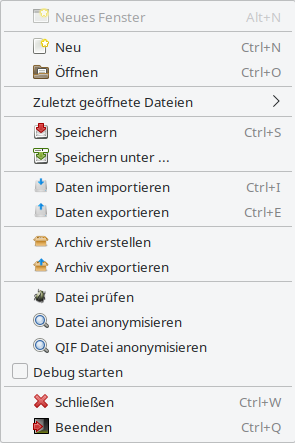
\includegraphics[width=1\textwidth]{image/screenshot/home_menubar_file}
	\vspace{-10pt}					% space between the floating and the caption below the floating
	\captionsetup{
		type=figure,%				% define "figure" or "table" type, mandatory
		name=Abb.,%					% rename label caption, default="Figure" (or "Table")
		labelsep=newline}			% define the separator between the label and the caption text
	\caption{Menü \menus{Datei}}	% \caption is mandatory to reference a figure in lof
	%\vspace{30pt}					% space below the caption
	\label{home_menubar_file}
\end{minipage}

\begin{itemize}
	\item \menus{Speichern}: Speichert Änderungen in der aktuellen Grisbi Datei (Tastenkombination \keys{Ctrl+S});%\menus{Save}: Saves the current account file (shortcut \keys{Ctrl+S});%\menus{Enregistrer}: enregistre le fichier de comptes en cours (raccourci-clavier \keys{Ctrl+S});
	\item \menus{Speichern unter ...}: Öffnet einen Dateimanager, um die Datei der aktuellen Konten unter einem Namen und an einem Ort Ihrer Wahl zu speichern; Grisbi verwendet standardmäßig das aktuelle Verzeichnis, den Namen der Datei der aktuellen Konten und die \gls{Dateinamenserweiterung} \file{.gsb};%\menus{Save As}: opens a file manager to save the current accounts file with the name and location of your choice; Grisbi defaults to the current directory, the name of the current accounts file, with the \file{.gsb} extension;%\menus{Enregistrer sous}: ouvre un gestionnaire de fichiers pour enregistrer le fichier de comptes en cours avec le nom et à l'emplacement de votre choix; Grisbi vous propose par défaut le répertoire courant, le nom du fichier de comptes en cours, avec l'\gls{extension} \file{.gsb};
	\item \menus{Daten importieren}: Startet den Assistent \dequote{Daten importieren} einer anderen Software (Tastenkombination \keys{Strg+I}); Sehen \vref{move-import-importinit}%\menus{Import file...}: starts the \enquote{Importing transactions into Grisbi} wizard of another software (shortcut \keys{Ctrl+I}); see \vref{move-import-importinit};%\menus{Importer un fichier}: démarre l'assistant d'importation de fichiers d'un autre logiciel (raccourci-clavier \keys{Ctrl+I}); voir la section \vref{move-import-importinit};
	\item \menus{Daten exportieren}: Startet den Assistent \dequote{Konten exportieren} (Tastenkombination \keys{Strg+E}); Sehen \vref{move-export};%\menus{Export accounts as QIF/CSV file}: starts the \enquote{Exporting Grisbi accounts} wizard (shortcut \keys{Ctrl+E}); see \vref{move-export};%\menus{Exporter vers un fichier QIF/CSV}: démarre l'assistant d'exportation de fichiers de compte (raccourci-clavier \keys{Ctrl+E}); voir la section \vref{move-export};	
	\item \menus{Archiv erstellen}: Startet den Assistent Archive erstellen; Sehen \vref{datamanagement-history-new};%\menus{Archive transactions}: starts the archive creation wizard; see \vref{datamanagement-history-new};%\menus{Créer une archive}: démarre l'assistant de création d'archive; voir la section \vref{datamanagement-history-new};	
	\item \menus{Archiv exportieren}: Startet den Assistent Archive exportieren; Sehen \vref{datamanagement-history-export};%\menus{Export an archive as GSB/QIF/CSV file}: starts the archive export wizard; see \vref{datamanagement-history-export};%\menus{Exporter une archive vers un fichier GSB/QIF/CSV}: démarre l'assistant d'exportation d'archive; voir la section \vref{datamanagement-history-export};
	\item \menus{Datei prüfen}: Startet den Assistent Konsistenzprüfung, die Ihnen helfen wird, nach Unstimmigkeiten in Ihrer Kontodatei zu suchen; Sehen \vref{maintenance-file-debug}%\menus{Debug account file}: starts the debug wizard for this file, which will help you look for inconsistencies in your account file; see \vref{maintenance-file-debug};%\menus{Déboguer le fichier de comptes}: démarre l'assistant de débogage de ce fichier, qui va vous aider à chercher des incohérences dans votre fichier de comptes; voir la section \vref{maintenance-file-debug};
	\item \menus{Datei anonymisieren}: Startet den Assistent \dequote{Grisbi Datei anonymisieren}, der eine anonyme Kopie Ihrer Kontodatei erstellt; diese Datei kann an einen Fehlerbericht angehängt werden;%\menus{Obfuscate account file}: starts the wizard that produces an anonymous copy of your account file; this file can be attached to a bug report; see \vref{maintenance-file-anonymous};%\menus{Rendre anonyme le fichier de comptes}: démarre l'assistant qui produit une copie anonymée (de manière irréversible) de votre fichier de comptes; ce fichier pourra être joint à un rapport de bogue; voir la section \vref{maintenance-file-anonymous};	
	\item \menus{\gls{QIF} Datei anonymisieren}: Startet den Assistent QIF Datei anonymisieren, der eine anonyme Kopie dieser Datei erstellt; diese Datei kann an einen Fehlerbericht angehängt werden; Sehen \vref{maintenance-QIF-anonymous};%\menus{Obfuscate QIF file}: starts the wizard that produces an anonymous copy of this file; this file can be attached to a bug report; see \vref{maintenance-QIF-anonymous};%\menus{Rendre anonyme le fichier QIF}: démarre l'assistant qui produit une copie anonymée (de manière irréversible) de ce fichier; ce fichier pourra être joint à un rapport de bogue; voir la section \vref{maintenance-QIF-anonymous};	
	\item \menus{Debug starten}: Aktiviert den Debug Modus, der eine Protokolldatei der Ereignisse erstellt; Sehen \vref{maintenance-debug-mode} %\menus{Debug mode}: puts Grisbi in debug mode, which creates a log file of events; see \vref{maintenance-debug-mode};%\menus{Mode de débogage}: met Grisbi en mode de débogage, qui crée un fichier-journal des évènements; voir la section \vref{maintenance-debug-mode}; 	
	\item \menus{Schließen}: Schließt die aktuell geöffnete Grisbi Datei; Grisbi bietet Ihnen an, sie zu speichern, falls Sie dies noch nicht getan haben (Tastenkombination \keys{Strg+W}). %\menus{Close}: closes the current accounts file; Grisbi offers to save it if you have not already done it (shortcut \keys{Ctrl+W});%\menus{Fermer}: ferme le fichier de comptes en cours; Grisbi vous propose de l'enregistrer si ce n'est déjà fait (raccourci-clavier \keys{Ctrl+W});
	\item \menus{Beenden}: Beendet Grisbi; Grisbi wird Sie zunächst auffordern, die Kontendatei zu speichern, falls Sie dies noch nicht getan haben (Tastenkombination \keys{Strg+Q}).%\menus{Quit}: close Grisbi; Grisbi will first ask you to save the accounts file, if you have not already done so (shortcut \keys{Ctrl+Q});%\menus{Quitter}: ferme Grisbi; Grisbi vous propose auparavant d'enregistrer le fichier de comptes, si ce n'est pas déjà fait (raccourci-clavier \keys{Ctrl+Q}).
\end{itemize}


\subsection{Menü \menus{Bearbeiten}\label{home-menus-edit}}

\textbf{Notiz}: Im Menü Bearbeiten sind einige Einträge erst aktiv wenn ein Konto oder eine Buchung ausgewählt wird.

Dieses Menü enthält die folgenden Funktionen:%This menu includes the following functions:

\vspace{3mm}
\noindent
\begin{minipage}{.7\linewidth}
	\begin{itemize}[rightmargin=.6cm]
		\item \menus{Buchung bearbeiten}: ermöglicht es, einen ausgewählten Vorgang zu korrigieren, siehe Abschnitt \vref{transactions-modify}, \menus{Modification d'une opération};%TODO to translate
		% allows a selected operation to be rectified, see section \vref{transactions-modify}, \menus{Modification d'une opération};%TODO to translate
		%\menus{Éditer l'opération}: permet la rectification d'une opération existante, voir la section \vref{transactions-modify}, \menus{Modification d'une opération};
		\item \menus{Buchung erstellen}: ermöglicht die Erstellung einer neuen Transaktion in einem Konto (Tastenkombination \keys{Strg+T}), siehe den Abschnitt \vref{transactions-new}, \menus{Saisie d'une nouvelle opération};%TODO to translate
		% allows the creation of a new transaction in an account (shortcut \keys{Ctrl+T}), see the section \vref{transactions-new}, \menus{Saisie d'une nouvelle opération};%TODO to translate
		%\menus{Nouvelle opération}: permet la création d'une nouvelle opération dans un compte (raccourci-clavier \keys{Ctrl+T}), voir la section \vref{transactions-new}, \menus{Saisie d'une nouvelle opération};
		\item \menus{Buchung löschen}: löscht einen ausgewählten Vorgang, siehe Abschnitt \vref{transactions-delete}, \menus{Deleting a transaction};%TODO to translate
		% deletes a selected operation, see section \vref{transactions-delete}, \menus{Deleting a transaction};
		%\menus{Supprimer une opération}: supprime une opération existante, voir la section \vref{transactions-delete}, \menus{Suppression d'une opération};
	\end{itemize}
\end{minipage}
\hspace{10pt}	
\begin{minipage}{.3\linewidth}
	\vspace{-5pt}					% space above the floating (minus intextsep=separation between float and text in text)
	\centering						% centering the floating figure in the "wrap"
	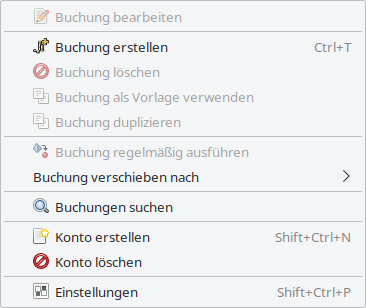
\includegraphics[width=1\textwidth]{image/screenshot/home_menubar_edit}
	\vspace{-15pt}					% space between the floating and the caption below the floating
	\captionsetup{
		type=figure,%				% define "figure" or "table" type, mandatory
		name=Abb.,%					% rename label caption, default="Figure" (or "Table")
		labelsep=newline}			% define the separator between the label and the caption text
	\caption{Menü \menus{Bearbeiten}}	% \caption is mandatory to reference a figure in lof
	%\vspace{30pt}					% space below the caption
	\label{home_menubar_edit}
\end{minipage}

\begin{itemize}
	\item \menus{Buchung als Vorlage verwenden}: Erstellt die Kopie eines ausgewählten Vorgangs, wobei das aktuelle Datum in das Buchungsformular eingetragen wird, siehe Abschnitt \vref{transactions-model}, \menus{Opération sélectionnée comme modèle};%TODO to translate
	%Use selected transaction as a template}: allows you to create a new operation from a selected operation, see \vref{transactions-model}, \menus{Selecting a transaction for use as a template}:
	%\menus{Utiliser l'opération sélectionnée comme modèle}: permet de créer une nouvelle opération à partir d'une opération sélectionnée, voir la section \vref{transactions-model}, \menus{Opération sélectionnée comme modèle};
	\item \menus{Buchung duplizieren}: Erstellt eine Kopie, die mit dem ausgewählten Buchung identisch ist, und öffnet das Buchungsformular, siehe Abschnitt \vref{transactions-duplicate}, \menus{Clone a transaction};%TODO to translate
	%\item \menus{Clone transaction}: is used to duplicate an existing operation, see section \vref{transactions-duplicate}, \menus{Clone a transaction};
	%\menus{Cloner l'opération}: permet de dupliquer une opération existante, voir la section \vref{transactions-duplicate}, \menus{Clonage d'une opération};
	\item \menus{Buchung regelmäßig ausführen}: siehe Abschnitt \vref{transactions-schedule}, \menus{Converting a transaction to a scheduled transaction};%TODO to translate
	%\item \menus{Convert to scheduled transaction}: see section \vref{transactions-schedule}, \menus{Converting a transaction to a scheduled transaction};
	%\menus{Convertir en opération planifiée}: voir la section \vref{transactions-schedule}, \menus{Conversion d'une opération en opération planifiée};
	\item \menus{Buchung verschieben nach}: Verschiebt die Buchung auf das ausgewählte Konto, siehe Abschnitt \menus{Moving a transaction to another account};%TODO to translate
	%\item \menus{Move transaction to another account}: see section \vref{transactions-move}, \menus{Moving a transaction to another account};
	%\menus{Déplacer l'opération vers un autre compte}: voir la section \vref{transactions-move}, \menus{Déplacement d'une opération vers un autre compte};
	\item \menus{Buchungen suchen}:
	\begin{itemize}
		\item Öffnet die Suche nach Buchungen mit der Funktionalität von Berichte wenn eine Registerkarte des Navigationsbereich ausgewählt ist, siehe Abschnitt \vref{reports-creation}, \menus{Création d'un état}>>>;%TODO to modify
		%opens the properties window for a report when a navigation panel tab is selected, <<<see chapter \vref{reports-creation}, \menus{Création d'un état}>>>;%TODO to modify
		%ouvre la fenêtre de propriétés d'un état quand un onglet du panneau de navigation est sélectionné, voir le chapitre \vref{reports-creation}, \menus{Création d'un état};
		\item Zeigt das Suchfeld an, wenn ein Konto oder eine Buchung ausgewählt wird, siehe Abschnitt <<<\vref{accounts-search}, \menus{alphanumerische Suche?}>>> TO CREATE; %TODO to create
		%displays the search box when an account or transaction is selected, <<<see chapter \vref{accounts-search}, \menus{alphanumeric search}>>> TO CREATE; %TODO to create
		%affiche la fenêtre de recherche quand un compte ou une opération est sélectionné, <<<voir le chapitre \vref{accounts-search}, \menus{Recherche alphanumérique}>>> A CRÉER; %TODO to create
	\end{itemize}
	\item \menus{Konto erstellen}: Startet den Assistent Konto erstellen für die Erstellung eines neuen Kontos in Ihrer Grisbi-Datei (Tastenkombination \keys{Shift+Ctrl+N}), siehe Abschnitt \vref{accounts-new}, \menus{Creating a new account};%TODO to translate
	%\item \menus{New account}: starts the wizard for creating a new account in your Grisbi file (shortcut \keys{Shift+Ctrl+N}), see section \vref{accounts-new}, \menus{Creating a new account};
	%\menus{Nouveau compte}: démarre l'assistant de	création d'un nouveau compte dans votre fichier Grisbi (raccourci-clavier \keys{Maj \shift+Ctrl+N}), voir la section \vref{accounts-new}, \menus{Création d'un nouveau compte};
	\item \menus{Konto löschen}: löscht das ausgewählte Konto aus Ihrer Grisbi-Datei, siehe Abschnitt \vref{accounts-delete}, \menus{Removing the current account};%TODO to translate
	%\item \menus{Remove current account}: deletes the selected account from your Grisbi file, see section \vref{accounts-delete}, \menus{Removing the current account}:
	%\menus{Supprimer le compte courant}: efface le compte sélectionné de votre fichier Grisbi, voir la section \vref{accounts-delete}, \menus{Suppression d'un compte};
	\item \menus{Einstellungen}: ermöglicht die Konfiguration von Grisbi (Tastenkombination \keys{Shift \shift+Strg+P}); siehe Kapitel \vref{setup}, \menus{Configuration of Grisbi}.%TODO to translate
	%\item \menus{Preferences}: allows you to configure Grisbi (shortcut \keys{Maj \shift+Ctrl+P}); see the chapter \vref{setup}, \menus{Configuration of Grisbi}.
	%\menus{Préférences}: permet de configurer Grisbi (raccourci-clavier \keys{Maj \shift+Ctrl+P}); voir le chapitre \vref{setup}, \menus{Configuration de Grisbi}.
\end{itemize}


\subsection{Menü \menus{Ansicht}\label{home-menus-display}}

\textbf{Notiz}: Im Menü \menus{Ansicht} sind die Einträge erst aktiv wenn ein Konto ausgewählt wird.%in the \menus{View} menu, entries are only active when an account is selected.

Dieses Menü enthält die folgenden Funktionen:%This menu includes the following functions: 

\vspace{3mm}
\noindent
\begin{minipage}{.7\linewidth}
	\begin{itemize}[rightmargin=.6cm]
	\item \menus{Buchungsformular anzeigen}: öffnet das Buchungsformular für das ausgewählte Konto;
	%Show transaction form}: expands the Transaction/Scheduled form for the selected account;
	%Montrer le formulaire de saisie des opérations}: permet de développer le formulaire de saisie des opérations du compte sélectionné;
	\item \menus{Abgestimmte Buchungen anzeigen}: zeigt die abgestimmten Buchungen für das ausgewählte Konto (Tastenkombination \keys{Alt+R});
	%Show reconciled}: displays reconciled transactions for the selected account (shortcut \keys{Alt+R});
	%Montrer les opérations rapprochées}: permet l'affichage des opérations rapprochées du compte sélectionné (raccourci-clavier \keys{Alt+R});
	\item \menus{Erstellte Archive anzeigen}: zeigt die Archivzeilen für das ausgewählte Konto (Tastenkombination \keys{Alt+L});
	%Show lines archives}: displays the archive lines for the selected account (shortcut \keys{Alt+L});
	%Montrer les lignes d'archives}: affiche les lignes d'archives du compte sélectionné (raccourci-clavier \keys{Alt+L});
	\item \menus{Geschlossene \indexword{Konten anzeigen}}\index{Konto!anzeigen}: zeigt Konten an, die geschlossen und nicht gelöscht wurden, siehe Abschnitt \vref{accounts-properties}, \menus{??Account properties??}; %TODO to update
	%Show \indexword{closed accounts}}\index{closed!account}: displays account(s) that have been closed and not deleted, see section \vref{accounts-properties}, \menus{Account properties?};
	%\menus{Montrer les \indexword{comptes clos}}\index{compte!clos}: affiche le(s) compte(s) clos et non supprimé(s), voir la section \vref{accounts-properties}, \menus{Propriétés d'un compte};
	\end{itemize}
\end{minipage}
\hspace{10pt}	
\begin{minipage}{.3\linewidth}
	%\vspace{-10pt}					% space above the floating (minus intextsep=separation between float and text in text)
	\centering						% centering the floating figure in the "wrap"
	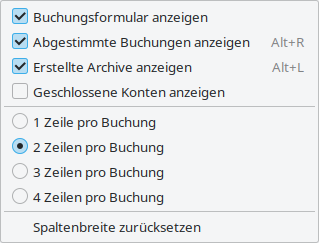
\includegraphics[width=1\textwidth]{image/screenshot/home_menubar_view}
	\vspace{-10pt}					% space between the floating and the caption below the floating
	\captionsetup{
	type=figure,%				% define "figure" or "table" type, mandatory
	name=Abb.,%					% rename label caption, default="Figure" (or "Table")
	labelsep=newline}			% define the separator between the label and the caption text
	\caption{Menü \menus{Ansicht}}		% \caption is mandatory to reference a figure in lof
	%\vspace{30pt}					% space below the caption
	\label{home_menubar_view}
\end{minipage}
\vspace{2mm}
\begin{addmargin*}[19pt]{0cm} 	% modify margin, * : left = right, [] = obligatory argument indentation, {} = optional argument left indentation 
Mit den folgenden vier Funktionen können Sie die Anzeige der Buchungen für das ausgewählte Konto konfigurieren:
%The following four functions can be used to configure the display of transactions for the selected account:
%Les quatres fonctions suivantes permettent de configurer l'affichage des opérations du compte sélectionné:
\end{addmargin*}
\vspace{-2mm}
\begin{itemize}
	\item \menus{1 Zeile pro Buchung};%Show one line per transaction}%Montrer une ligne par opération};
	\item \menus{2 Zeilen pro BuchungShow};%two lines per transaction}%Montrer deux lignes par opération};
	\item \menus{3 Zeilen pro BuchungShow};%three lines per transaction}%Montrer trois lignes par opération};
	\item \menus{4 Zeilen pro BuchungShow};%four lines per transaction}%Montrer quatre lignes par opération};
	\vspace{2mm}
	\begin{addmargin*}[-10pt]{0cm} 	% modify margin, * : left = right, [] = obligatory argument indentation, {} = optional argument left indentation 
	Und schließlich die letzte Funktion im Menü Ansicht:
	%And finally, the last function in the view menu:%Et enfin la dernière fonction du menu d'affichage:
	\end{addmargin*}	
	\item \menus{Spaltenbreite zurücksetzen}: In der Buchungsübersicht die Spaltenbreiten mit der Standardbreite anzeigen.
	%Reset the column width}: allows you to reset the columns of the tranaction lists to their original width. 
	%Réinitialiser la largeur des colonnes}: permet de remettre les colonnes des listes d'opérations du compte sélectionné ou de l'échéancier à leur largeur d'origine.
\end{itemize}

%TODO following
\subsection{\menus{Help} menu\label{home-menus-help}}

Most of the choices in this menu give links to websites. In order for these links to work, you must have specified to Grisbi the navigation software (or browser) that you wish to use, in the \menus{Edit - Preferences} (see \vref{setup-general-programs}, \menus{Programmes}). The \menus{Help} menu includes the following choices\footnote{\strong{Translators Note:} A "help us with translation" menu item is mentioned in the French version of the manual but does note appear in the English version of Grisbi at release 1.0}:

\begin{itemize}
	\item \menus{Manual}: opens your browser to the  \dequote{Grisbi User Manual page} (shortcut key  \key{Ctrl}\key{H});
	\item \menus{Quick start}: opens your browser to the  \dequote{Grisbi Quick Start page};
%	\item \menus{Traduction}: opens your browser to the \dequote{Translate Grisbi}, to help us to widen the internationalization of Grisbi;
	\item \menus{About Grisbi...}: displays the program information box: you will find details about the version, the link to Grisbi's site, the acknowledgements page (contributors to the project) and the user license;
	\item \menus{Grisbi website}: opens your browser to the \lang{Grisbi}\footnote{\urlGrisbi{}} web site;
	\item \menus{Report a bug}: opens your browser to the \lang{Grisbi Bug Tracker page}\footnote{\urlBugTracker{}} to allow you to report a bug that you have discovered. You can also follow on this page the evolution of the corrections made to the reported bugs;
	\item \menus{Tip of the day}: opens a dialog box that displays a tip of use, different each time Grisbi starts; you can successively display all the tips, and choose whether or not the display of the tip of the day when starting Grisbi. To remove or reactivate the tip of the day, see \vref{setup-display-messages-trick}, \menus{Tip of the day}.
\end{itemize}


\section{Shortcut keys\label{home-shortcuts}}


Keyboard shortcuts make it easy to enter data and navigate through Grisbi's windows, avoiding the need to move and click. By using the ones corresponding to the most common manipulations for you, you improve your \indexword{ergonomics}\index{ergonomie} by limiting the important movements of your arms.
 
Grisbi has a number of keyboard shortcuts, presented here according to different themes (see also  \vref{introduction-manual-conventions}, \menus{Typographical conventions in this manual}).
.

\subsection{Application and files}

\begin{itemize}
	\item New accounts file: \key{Ctrl}\key{N}
	\item Open an account file: \key{Ctrl}\key{O}
	\item Register the account file: \key{Ctrl}\key{S}
	\item Close the account file: \key{Ctrl}\key{W}
	\item Close Grisbi: \key{Ctrl}\key{Q}
\end{itemize}


\subsection{Navigation panel}

\begin{itemize}
	\item Select a tab or account: \key{ Arrow Up}, \key{Arrow Down}, \key{Page Up} ou \key{Page Down}
\end{itemize}

\subsection{List of transactions and scheduled transactions}

\begin{itemize}
	\item Select a transaction: \key{Enter}
	\item Move selection:\key{Arrow Up} ou \key{Arrow Down}
	\item New transaction:  \key{Enter} on empty line, or \key{Ctrl}\key{T}
	\item Modify an transaction: \key{Enter}
	\item Delete an transaction: \key{Delete};
	\item Select a transaction for a reconciliation:\key{Ctrl}\key{P}
	\item Remove a reconciled transaction: \key{Ctrl}\key{R}
	\item Show or hide archival lines: \key{Altl}\key{L}
\end{itemize}


\subsection{Entry form}

\begin{itemize}
	\item The \key{Enter} is configurable: it can be set to either move in the input form, or to validate the entry
	\item Move to the next field: \key{Tab} (depending on your configuration choice)
	\item Cancel the current entry: \key{Esc}
	\item Accept auto-complete: \key{Tab} or \key{Enter} (depending on your configuration choice)
	\item  Euro symbol: \key{AltGr}\key{e}
\end{itemize}

\subsection{Drop down lists}

\begin{itemize}
	 \item Open a list: \key{Page Down} or \key{Down Arrow}
	 \item Move in the list: \key{Up Arrow}, \key{Down Arrow}, \key{Page Up} or \key{Page Down}
	 \item Validate a choice within a list: \key{Enter}
	 \item Currencies, ??exercises?? and methods of payment:
		\begin{itemize}
			\item open list: \key{Space}; 
			\item move in the list: \key{Up Arrow} or \key{Down Arrow};
			\item validate the item in the list: \key{Space}.
		\end{itemize}
\end{itemize}


\subsection{Dates entered on the calendar}

\begin{itemize}
	\item Opens a calendar (on the date field): \key{Ctrl}\key{Enter}
	\item Closes the calendar without changing the date: \key{Esc}
	\item Validate the selected date: \key{Enter}
	\item Next or previous day: \key{+} or \key{-}, \key{Right Arrow} or \key{Left Arrow}
	\item Previous or next week: \key{Up Arrow} or \key{Down Arrow}
	\item Previous or next month: \key{Page Up} or \key{Page Down}
	\item First day or last day of the month: \key{Start} or \key{End}
\end{itemize}


\subsection{Dates entered on keyboard }

\begin{itemize}
	\item Next or previous day: \key{+} or \key{-}
	\item Previous or next week: \key{Shift} \key{+} or \key{Majuscule} \key{-}
	\item Previous or next month: \key{Page Up} or \key{Page Down}
	\item Previous or Next Year: \key{Shift} \key{Page Up} or \key{Shift} \key{Page Down}
	\item Validate the selected date \key{Enter}
\end{itemize}


\subsection{Payees, categories, budget allocations, credit simulator, historical data and forecasts}

\begin{itemize}
	\item Move selection: \key{Up Arrow}, \key{Down Arrow}, \key{Page Up} or \key{Page Down}
%Ces raccourcis ne fonctionnent plus:
%	\item afficher les sous-catégories ou sous-imputations budgétaires (sur une catégorie ou une imputation budgétaire): \key{Espace};
%	\item afficher les opérations des sous-catégories ou sous-imputations budgétaires (sur une sous-catégorie ou une sous-imputation budgétaire): \key{Espace}.
\end{itemize}


\subsection{States and Configuration}

\begin{itemize}
	\item Select another tab: \key{Up Arrow}, \key{Down Arrow}, \key{Page Up}, \key{Page Down}
	\item Navigate between the tab panel and the different options in the settings panel: \key{Tab}, \key{Up Arrow}, \key{Down Arrow}, \key{Left Arrow} and \key{Right Arrow}
\end{itemize}

\subsection{Help}

\begin{itemize}
	\item Open your browser on the Grisbi User Manual page \key{Ctrl}\key{H}
\end{itemize}













			% TODO update screenshots and text "home", uncomment when finished
%\cleardoubleemptypage

%\include{06-grisbi-manuel-QIF-de}			% TODO update screenshots and text "QIF", uncomment when finished
%\cleardoubleemptypage

%\include{07-grisbi-manuel-datamanagement-de}	% TODO update screenshots and text "datamanagement", uncomment when finished
%\cleardoubleemptypage

%\include{08-grisbi-manuel-accounts-de}		% TODO update screenshots and text "accounts", uncomment when finished
%\cleardoubleemptypage

%\include{09-grisbi-manuel-transactions-de}	% TODO update screenshots and text "transactions", uncomment when finished
%\cleardoubleemptypage

%\include{10-grisbi-manuel-reconciliation-de}	% TODO update screenshots and text "reconciliation", uncomment when finished
%\cleardoubleemptypage

%\include{11-grisbi-manuel-planned-de}		% TODO update screenshots and text "planned", uncomment when finished
%\cleardoubleemptypage

%\include{12-grisbi-manuel-search-de}			% TODO update screenshots and text "search", uncomment when finished
%\cleardoubleemptypage

%\include{13-grisbi-manuel-third-de}			% TODO update screenshots and text "third", uncomment when finished
%\cleardoubleemptypage

%\include{14-grisbi-manuel-categories-de}		% TODO update screenshots and text "categories", uncomment when finished
%\cleardoubleemptypage

%\include{15-grisbi-manuel-budgetlines-de}	% TODO update screenshots and text "budgetlines", uncomment when finished
%\cleardoubleemptypage

%\include{16-grisbi-manuel-financialyear-de}	% TODO update screenshots and text "financialyear", uncomment when finished
%\cleardoubleemptypage

%\include{17-grisbi-manuel-credit-de}			% TODO update screenshots and text "credit", uncomment when finished
%\cleardoubleemptypage

%\include{18-grisbi-manuel-budget-de}			% TODO update screenshots and text "budget", uncomment when finished
%\cleardoubleemptypage

%\include{19-grisbi-manuel-bankcardmanagement-de}	% TODO update screenshots and text "bankcardmanagement", uncomment when finished
%\cleardoubleemptypage

%\include{20-grisbi-manuel-association}		% fr version only
%\cleardoubleemptypage

%\include{21-grisbi-manuel-reports-de}			% TODO update screenshots and text "reports", uncomment when finished
%\cleardoubleemptypage

%\include{22-grisbi-manuel-reports-creation-de}	% TODO update screenshots and text "reports-creation", uncomment when finished
%\cleardoubleemptypage

%\include{23-grisbi-manuel-setup-de}				% TODO update screenshots and text "setup", uncomment when finished
%\cleardoubleemptypage

%\include{24-grisbi-manuel-maintenance-de}		% TODO update screenshots and text "maintenance", uncomment when finished
%\cleardoubleemptypage



%% Files editors not used anymore, so useless 
%%\include{grisbi-manuel-todo}
%%\cleardoubleemptypage
%
%% Files editors not used anymore, so useless 
%%\include{grisbi-manuel-problems}
%%\cleardoubleemptypage
%
%% Useless so don't include it
%%\include{grisbi-manuel-XML}
%
%% Useless so don't include it
%%\include{grisbi-manuel-FDL}


% Prints the index
\printindex


% Displays a note at the beginning of the glossary
\renewcommand{\glossarypreamble}{\textbf{Notiz}: die meisten Definitionen der Einträge in diesem Glossar stammen aus den gleichnamigen Artikeln der freien und kollaborativen Enzyklopädie \lang{Wikipédia}\footnote{\urlWikipedia{}}. Obwohl diese Texte verändert und an den besonderen Kontext dieses Glossars angepasst wurden, dankt der Autor Wikipedia für die Bereitstellung dieser Referenzen.\newline}


% Prints the glossary
% For pdf only; redefined in hva/macros.hva by an empty command in html
\printglossary[%				% print glossary
	toctitle={Glossar}%			% define glossary name in toc, doesn't work with \printglossaries
	]


\end{document}



